\documentclass[11pt]{article}

\usepackage{smoothing_paper}




%%%%%%%%%%%%%%%%%%%%%%%%%%%%%%%%chiheb commands

\newcommand{\ie}{\emph{i.e.}}
\newcommand{\eg}{\emph{e.g.}}
\newcommand{\cf}{\emph{cf.}}
\newcommand{\prob}[1]{\mathrm{P}\left(#1\right)}
\newcommand{\expt}[1]{\mathrm{E}\left[#1\right]}
\newcommand{\expth}[1]{\hat{\mathrm{E}}\left[#1\right]}



\newcommand{\rset}{\mathbb{R}}
\newcommand{\nset}{\mathbb{N}}
\newcommand{\zset}{\mathbb{Z}}



\newcommand{\PERIOD}{.}
\newcommand{\COMMA}{,}
\newcommand{\BIGSPACE}{\,\,\,\,\,\,\,}



\newcommand{\Ordo}[1]{{\mathcal{O}}\left(#1\right)}
\newcommand{\ordo}[1]{{o}\left(#1\right)}

%%%%%%%%%%%%%%%%%%%%%%%%%%%%%%%%%%%%%%%%%%%%%%%%%%%%%%%%%%%%%%%%%%%%%%%%
%%
%% DO WE RELLY NEED THE FOLLOWING??

%%  new margin
%%%%%%%%%%%%%%%%%%%%%%%%%%%%%%%%%%%%%%%%%%%
\pagestyle{plain}                                                      %%
%%%%%%%%%% EXACT 1in MARGINS %%%%%%%                                   %%
\setlength{\textwidth}{6.5in}     %%                                   %%
\setlength{\oddsidemargin}{0in}   %%   
\setlength{\evensidemargin}{0in}  %%        
\setlength{\textheight}{8.5in}    %%       
\setlength{\topmargin}{-0.2in}    %%   
\setlength{\headheight}{0in}      %%    
\setlength{\headsep}{0in}         %%                   
\setlength{\footskip}{.5in}       %%                       
%%%%%%%%%%%%%%%%%%%%%%%%%%%%%%%%%%%%                                   %%
\newcommand{\required}[1]{\section*{\hfil #1\hfil}}                    %%
\renewcommand{\refname}{\hfil References Cited\hfil}                   %%

\def\SMALLSKIP{\smallskip}
\def\MEDSKIP{\medskip}
\def\BIGSKIP{\bigskip}

%%
%%%%%%%%%%%%%%%%%%%%%%%%%%%%%%%%%%%%%%%%%%%%%%%%%%%%%%%%%%%%%%%%%%%%%

\makeatletter
\def\BState{\State\hskip-\ALG@thistlm}
\makeatother



%%%%%%%%%%%%%%%%%%%%%%%%%%%%%%%%%%%%%%%%

\title{Efficient option pricing for Rough Bergomi model} 
    \date{ }

\begin{document}
\maketitle


\section{The goal and outline of the project}
The main goal of the project is to design a fast option pricer, based on multi-index stochastic collocation (MISC), for options whose dynamics follow rBergomi model.
\section{The rBergomi model}\label{sec:The rBergomi model}

We use  the rBergomi model for the price process $S_t$ as defined in  \cite{bayer2016pricing}, which is defined by

\begin{align}\label{eq:rBergomi_model1}
	dS_t = \sqrt{v_t} S_t dZ_t,\\
	v_t = \xi_0(t) \exp\left( \eta \tilde{W}_t - \frac{1}{2} \eta^2 t^{2H} \right),
\end{align}
where for $0 < H < 1$,  we have $\tilde{W}^H $ is a certain Volterra process,  defined by
\begin{align}
	\tilde{W}_t^H = \int_0^t K(t,s) dW_s^1, \quad K(t,s) = \sqrt{2H} (t-s)^{H - 1/2}.
\end{align}


$W_1, Z$ denote two \emph{correlated} standard Brownian motions with correlation $\rho$, so that
\begin{align}
	Z:=\rho	W_1+ \bar{\rho}W_2 \equiv \rho W_1+\sqrt{1-\rho^2} W_2
\end{align}

Therefore, Eq \ref{eq:rBergomi_model1} can be written as 

\begin{align}\label{eq:rBergomi_model}
	S_t&= S(0)  \operatorname{exp}\left( \int_{0}^{t} \sqrt{v(s)} dZ(s)- \frac{1}{2} \int_{0}^{t} v(s) ds   \right)     \nonumber\\
	v(u)&=\xi_0(u) \operatorname{exp}\left( \eta \tilde{W}_u^H- \frac{\eta^2}{2} u^H \right) .
\end{align}

We refer to $v_u$ as the variance process, where $\xi_0(u) = \expt{v_u} \in \mathcal{F}_0$ a.s. the forward variance curve. 

$\tilde{W}^H $ is a centered, locally $(H-\epsilon)$- H\" \o lder continuous, Gaussian process with $\var{\tilde{W}^H_t} = t^{2H}$.


In \cite{bayer2016pricing}, the  approach consists in sampling the Gaussian process $Z$ and $\tilde{W}^H$ on a discrete time grid using exact simulation and then approximating $S$ and $v$ using Euler  discretization.

Assuming $S_0 = 1$, and using the conditioning argument on the $\sigma$-algebra generated by $W_1$ (argument first used by \cite{romano1997contingent} in the context of Markovian SV
models), we can  show that the call price is given by

\begin{align}\label{BS_formula_rbergomi}
	C_{RB}\left( T, K \right) &= E\left[ \left(S_T - K \right)^+ \right]  \nonumber\\
	&=\expt{\expt{(S_T-K)^+ \mid \sigma(W^1(t) ,t \le T)}}\nonumber \\
	&=E\left[C_{BS}\left( S_0 = \operatorname{exp}\left(\rho \int_0^T \sqrt{v_t} dW_t^1 - \frac{1}{2}
	\rho^2 \int_0^T v_t dt\right),\ K = K, \ T = 1, \ \sigma^2 = (1-\rho^2)
	\int_0^T v_t dt \right) \right],
\end{align}
where $C_{BS}$ denotes the Black-Scholes price.

In fact, if we use the orthogonal decomposition of $S_t$ into $S_{t}^1$ and $S_{t}^2$, where

\begin{align}
	S_t^1:=\mathcal{E}\{ \rho \int_{0}^{t}  \sqrt{v_s} dW_s^1\}, \: S_t^2:= \mathcal{E}\{ \sqrt{1-\rho^2} \int_{0}^{t}  \sqrt{v_s} dW_s^2  \}	,
\end{align}

where $\mathcal{E}()$ denotes the stochastic exponential, then, we obtain
\begin{align}
	\log S_t \mid \mathcal{F}_t^1 \sim \mathcal{N}\left( \log S_t^1-\frac{1}{2} (1-\rho^2) \int_{0}^{t} v_s ds , (1-\rho^2) \int_{0}^{t} v_s ds \right),
\end{align} 

where $\mathcal{F}_t^1= \sigma\{ W_s^1: s\le t\}$. Therefore, we obtain \eqref{BS_formula_rbergomi}.


The main challenge is the computation of $S=\int_{0}^{T} \sqrt{v_t} dW_t^1$ and $V=\int_{0}^{T} v_t dt$. As was mentioned in \cite{bayer2017regularity}, we may try to
avoid any sampling related to $W^2$ by   a brute-force approach that  consists in simulating a scalar Brownian motion $W^1$, followed by computing  $\tilde{W}^H= \int K dW^1$  by It\^o/Riemann Stieltjes approximations of $(S,V)$. However, this is not advisable given the singularity of the Volterra kernel $K$. Therefore,  one needs to simulate the two-dimensional Gaussian process $(W_t^1, \tilde{W}^H_t: 0 \le t \le T)$.
\section{Numerical examples}


\subsection{Numerical tests description}
For our numerical tests, we coupled the C++ implementation used in \cite{bayer2016pricing} with the MISC library, and for comparison purposes we compare our results to the python code used in \cite{mccrickerd2017turbocharging} with MC method, for $M=10^7$ paths. We note that both used methods have similar complexity for constructing the spot prices which is of order $\Ordo{N \log(N)}$. Also, we use $S_0=1$, so the options will be prices in terms of the moneyness $K$, where $K$ is the strike price.

We start our numerical tests by comparing the values of call options  prices for different values of strikes $K=\{1.2, 1,0.8, e^{-4}\} $ for $H=0.43$ (we note that this value of $H$ is not realistic but it is a good starting point since this case the fractional Brownian motion (fBm) becomes simply Brownian motion) and $K=\{1.2, 1,0.8\} $ for $H=0.07$  in Section \ref{sec:Comparing call options prices rbergomi}. The used parameters are $H=\{0.43, 0.07\},\: \eta=1.9, \: \rho=-0.9,\: T=1$ and $\xi_0=0.235^2$. The values between parentheses in the tables are the standard errors for MC method. The results were reported for number of time steps $N \in \{2,4,8,16\}$. We note that we may need higher number of time steps $N$ to  achieve better accuracy but since  we believe that we have order one convergence with respect to $\Delta t$ (which is the limiting factor in the convergence), it is no so bad to test for few time steps. We  are later going to use the Richardson extrapolation, which we  hope to improve the convergence to  quadratic (see figure  \ref{fig:rBergomi_weak_error} which shows that  the weak error does not seem too bad already at this number of time steps).








\begin{figure}[!h]
	\begin{center}
		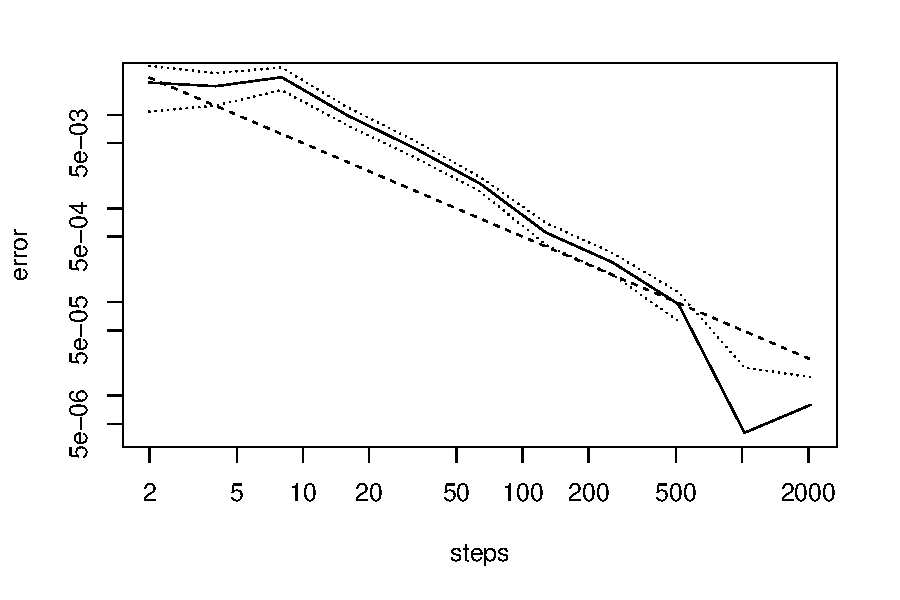
\includegraphics[scale=0.5]{./figures/rBergomi_weak_error/weak_RT.pdf}
		\caption{The weak error of rBergomi model}
		\label{fig:rBergomi_weak_error}
	\end{center}
\end{figure}

We note that for some cases, the convergence becomes extremely slow (either the bias stagnates at one value or it keeps increasing or decreasing without reaching the prescribed tolerance) specially when we are close to at-the money option ($K$ close to 1), we do not put values for those cases. We also remark that we have better agreement between the results of MISC coupled with the C++ code and the MC method using the python code form \cite{mccrickerd2017turbocharging}, for small values of moneyness.

In Section \ref{sec:Convergence plots using MISC_H_043}, we show the convergence plots given by MISC library for the cases of $K=\{e^{-4},1.2\}$ and $H=0.43$. We emphasize that in each case we have $2N$ stochastic parameters, the first $N$ correspond to $W_u^1$, while the last $N$ stochastic parameters correspond to $W_u^2$. Table \ref{table: Complexity rates for different number of time steps_rbergomi} summarizes the obtained complexity rates for different number of time steps (for more details, see Section \ref{sec:Convergence plots using MISC_H_043}. For other cases, we could not obtain the convergence rates as we explained in the paragraph above. The table \ref{table: Complexity rates for different number of time steps_rbergomi} supports our observation that for values of $K$ close to at the money ($K=1$), we observe a bad convergence behavior of MISC. In fact, the rates are much worse for $K=1.2$ than $K=e^{-4}$. If we look at Section \ref{sec:Convergence plots using MISC_H_043}, we may see a potential explanation for this different complexity behavior with respect to $K$. In fact, it is clear by comparing the plots of  the convergence rate of mixed differences per level for different value of $K$ and  the same number of time steps, we may notice that the convergence of mixed differences is much faster for the case of $K=e^{-4}$ than $K=1.2$. This observation is supported by external tests (See Section \ref{sec:mixed differences rbergomi}), where we compare the convergence of first and second differences for $K=e^{-4},=1.2$, for $8$ and $16$ time steps for $H=0.43,0.07$. \red{We still do not have a clear explanation why the rates are sensitive to the values of $K$.}

\begin{table}[h!]
	\centering
	\begin{tabular}{l*{6}{c}r}
		Method \textbackslash  Steps             & $2$ & $4$ & $8$  & $16$   \\
		\hline
		without Richardson  extrapolation $(K=e^{-4})$ & $-3/20$ & $-8/25$ & $-4/5$ & $- 13/10$  \\
		without Richardson  extrapolation $(K=1.2)$ & $-13/20$ & $-9/10$ & $-5/4$ & $-$  \\
		\hline
	\end{tabular}
	\caption{Complexity rates for different number of time steps for $H=0.43$ and $K=\{e^{-4},1.2\}$}
	\label{table: Complexity rates for different number of time steps_rbergomi}
\end{table}


\subsection{Comparing call options prices }\label{sec:Comparing call options prices rbergomi}
\subsubsection*{Case $H=0.43$}
\begin{table}[h!]
	\centering
	\begin{tabular}{l*{6}{c}r}
		Method \textbackslash  Steps            & $2$ & $4$ & $8$ & $16$  \\
		\hline
		MISC ($TOl=10^{-1}$)  & $0.1057$ & $0.0988$ & $0.0836$ & $0.0594$  \\
		MISC ($TOl=10^{-2}$)  & $0.1113$ & $0.0939$ & $0.0820$ & $-$  \\
		MISC ($TOl=10^{-3}$)        & $0.1081$ &$0.0918$ &  $0.0822$ &  $-$ \\
		MISC ($TOl=10^{-4}$)    & $0.1080$ & $0.0921$  & $-$ & $-$  \\
		%				MC method ($M=10^{6}$)    & $0.0840$ & $0.0781$  & $0.0746$ & $0.0729$  \\
		MC method ($M=10^{7}$)   & $\underset{(4.14e-05)}{0.0840}$ & $ \underset{(3.23e-05)}{0.0782}$  & $ \underset{(2.84e-05)}{0.0748}$ & $ \underset{(8.36e-06)}{0.0729}$ \\		
		
		\hline
	\end{tabular}
	\caption{ Call option price of the different methods for different number of time steps. Case $K=1$}
	\label{table: Call option price of the different methods for different number of time steps. Case $K=1$}
\end{table}

%\begin{table}[h!]
%	\centering
%	\begin{tabular}{l*{6}{c}r}
%		Method \textbackslash  Steps            & $2$ & $4$ & $8$ & $16$  \\
%		\hline
%		MISC ($TOl=10^{-1}$)  & $0.6214$ & $0.6234$ &  $0.6250$ &  $0.6257$  \\
%		MISC ($TOl=10^{-2}$)  &  $0.6214$ &  $0.6234$ &  $0.6293$ & $ 0.6314$  \\
%		MISC ($TOl=10^{-3}$)        &  $0.6338$ & $0.6348$ &   $-$ &  $-$ \\
%		MISC ($TOl=10^{-4}$)    &  $-$ &  $0.6342$  & $-$ & $-$  \\
%%		MC method ($M=10^{6}$)    &  $0.6326$ &  $0.6332$  &  $0.6330$ &  $0.6337$  \\
%		MC method ($M=10^{7}$)   &  $0.6326$ &  $0.6331$  &  $0.6335$ &  $0.6336$  \\		
%		\hline
%	\end{tabular}
%	\caption{ Call option price of the different methods for different number of time steps. Case $K=e^{-1}$}
%	\label{table: Call option price of the different methods for different number of time steps. Case $K=e^{-1}$}
%\end{table}
%



\begin{table}[h!]
	\centering
	\begin{tabular}{l*{6}{c}r}
		Method \textbackslash  Steps            & $2$ & $4$ & $8$ & $16$  \\
		\hline
		MISC ($TOl=10^{-1}$)  & $0.2230$ & $0.2122$ &  $0.2038$ &  $0.1993$  \\
		MISC ($TOl=10^{-2}$)  &  $0.2373$ &  $0.2355$ &  $0.2274$ & $ -$  \\
		MISC ($TOl=10^{-3}$)        &  $0.2403$ & $0.2331$ &   $-$ &  $-$ \\
		MISC ($TOl=10^{-4}$)    &  $0.2405$ &  $0.2333$  & $-$ & $-$  \\
		%		MC method ($M=10^{6}$)    &  $0.6326$ &  $0.6332$  &  $0.6330$ &  $0.6337$  \\
		MC method ($M=10^{7}$)   & $\underset{(5.81e-05)}{0.2228}$ & $ \underset{(4.99e-05)}{0.2237}$  & $ \underset{(4.63e-05)}{0.2238}$ & $\underset{(1.41e-05)}{0.2236}$ \\		
		\hline
	\end{tabular}
	\caption{ Call option price of the different methods for different number of time steps. Case $K=0.8$}
	\label{table: Call option price of the different methods for different number of time steps. Case $K=0.8$}
\end{table}


\begin{table}[h!]
	\centering
	\begin{tabular}{l*{6}{c}r}
		Method \textbackslash  Steps            & $2$ & $4$ & $8$ & $16$  \\
		\hline
		MISC ($TOl=10^{-1}$)  & $0.0271$ & $0.0119$ &  $0.0044$ &  $0.0017$  \\
		MISC ($TOl=10^{-2}$)  &  $0.0352$ &  $0.0133$ &  $0.0048$ & $0.0017$  \\
		MISC ($TOl=10^{-3}$)        &  $0.0345$ & $0.0183$ &   $0.0093$ &  $0.0054$ \\
		MISC ($TOl=10^{-4}$)    &  $0.0347$ &  $0.0181$  & $0.0096$ & $-$  \\
		%		MC method ($M=10^{6}$)    &  $0.6326$ &  $0.6332$  &  $0.6330$ &  $0.6337$  \\
		MC method ($M=10^{7}$)   & $\underset{(2.41e-05)}{0.0184}$ & $ \underset{(1.28e-05)}{0.0105}$  & $\underset{(8.11e-06)}{0.0063}$ & $\underset{(1.89e-06)}{0.0043}$  \\	
		\hline
	\end{tabular}
	\caption{ Call option price of the different methods for different number of time steps. Case $K=1.2$}
	\label{table: Call option price of the different methods for different number of time steps. Case $K=1.2$}
\end{table}




%\begin{table}[h!]
%	\centering
%	\begin{tabular}{l*{6}{c}r}
%		Method \textbackslash  Steps            & $2$ & $4$ & $8$ & $16$  \\
%		\hline
%		MISC ($TOl=10^{-1}$)  & $0.8529$ & $0.8559$  &  $0.8529$  &  $0.8582$   \\
%		MISC ($TOl=10^{-2}$)  & $0.8529$  & $0.8559$  &  $0.8559$  & $0.8638$   \\
%		MISC ($TOl=10^{-3}$)        & $0.8529$  & $0.8648$  &   $0.8649$  & $0.8648$  \\
%		MISC ($TOl=10^{-4}$)    &  $0.8648$  &   $0.8647$   & $-$ & $-$  \\
%%		MC method ($M=10^{6}$)    &  $0.8646$  &   $0.8647$   &   $0.8643$  &   $0.8646$   \\
%		MC method ($M=10^{7}$)   &  $0.8646$  &  $0.8647$   &   $0.8648$  &  $0.8648$   \\		
%		\hline
%	\end{tabular}
%	\caption{ Call option price of the different methods for different number of time steps. Case $K=e^{-2}$}
%	\label{table: Call option price of the different methods for different number of time steps. Case $K=e^{-2}$}
%\end{table}
%




\begin{table}[h!]
	\centering
	\begin{tabular}{l*{6}{c}r}
		Method \textbackslash  Steps            & $2$ & $4$ & $8$ & $16$  \\
		\hline
		MISC ($TOl=10^{-1}$)  & $0.9699$ & $0.9730$  &  $0.9745$  &  $0.9752$ \\
		MISC ($TOl=10^{-2}$)  & $0.9699$ & $0.9730$  &  $0.9789$  &  $0.9809$ \\
		MISC ($TOl=10^{-3}$)         & $0.9699$ & $0.9818$  &  $0.9818$  &  $0.9819$ \\
		MISC ($TOl=10^{-4}$)     & $0.9816$ & $0.9817$  &  $0.9817$  &  $-$ \\
		%		MC method ($M=10^{6}$)   & $0.9816$ & $0.9817$  &  $0.9813$  &   $0.9815$ \\
		MC method ($M=10^{7}$)   & $0.9816$ & $0.9817$  &  $0.9817$  &   $0.9817$ \\	
		\hline
	\end{tabular}
	\caption{ Call option price of the different methods for different number of time steps. Case $K=e^{-4}$}
	\label{table: Call option price of the different methods for different number of time steps. Case $K=e^{-4}$}
\end{table}


Since we observed that it is difficult for MISC to converge for $N=4,8,16$ for small tolerances $TOL=10^{-3}, TOL=10^{-4}$, we plot the final payoff we are using to check if we have a problem of regularity (See figures (\ref{fig:rBergomi_payoff_4steps_wrt_monyeness_H_043_1}, \ref{fig:rBergomi_payoff_4steps_wrt_monyeness_H_043_2}) for $H=0.43$ and figures (\ref{fig:rBergomi_payoff_4steps_wrt_monyeness_1}, \ref{fig:rBergomi_payoff_4steps_wrt_monyeness_2}) for $H=0.07$). I think the problem we observed is not related to regularity.
\begin{figure}[!h]
	\centering
	\begin{subfigure}{.5\textwidth}
		\centering
		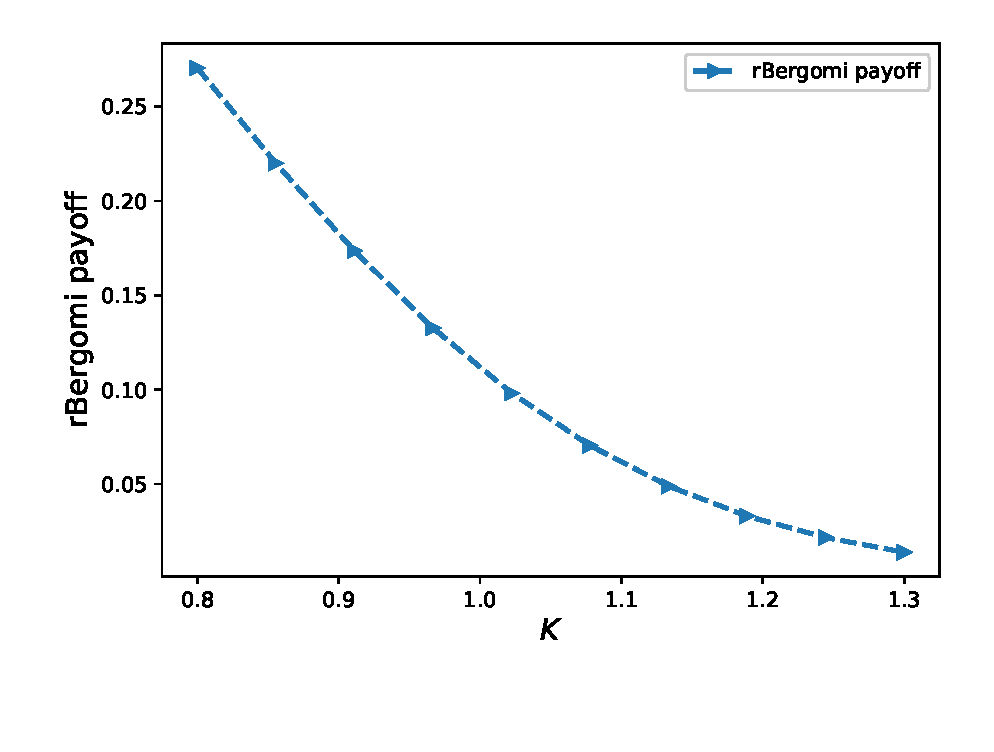
\includegraphics[width=0.95\linewidth]{./figures/payoff_plots_H_043/rBergomi_payoff_2steps_wrt_monyeness_2_H043}
		\caption{}
		\label{fig:rBergomi_payoff_4steps_wrt_monyeness_043_sub1}
	\end{subfigure}%
	\begin{subfigure}{.5\textwidth}
		\centering
		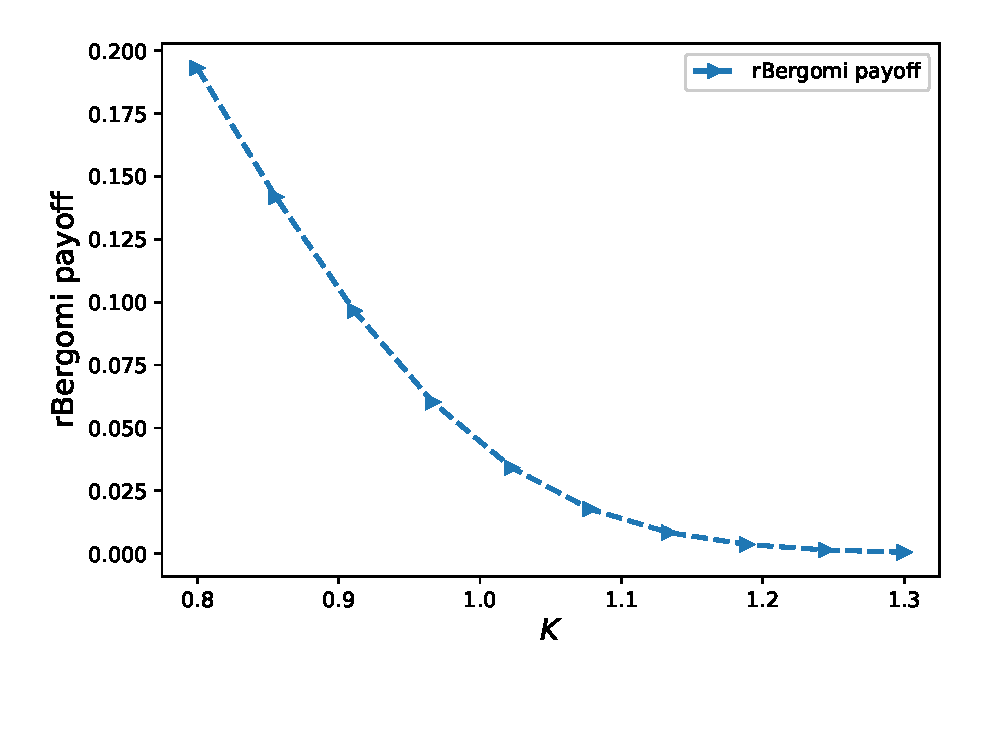
\includegraphics[width=0.95\linewidth]{./figures/payoff_plots_H_043/rBergomi_payoff_4steps_wrt_monyeness_2_H043}
		\caption{ }
		\label{fig:rBergomi_payoff_4steps_wrt_monyeness_043_sub2}
	\end{subfigure}%
	\caption{Black Scholes payoff for rBergomi model as a function of moneyness for $H=0.43$ a) $2$  time steps, b) $4$  time steps.}
	\label{fig:rBergomi_payoff_4steps_wrt_monyeness_H_043_1}
\end{figure}

\begin{figure}[!h]
	\centering
	\begin{subfigure}{.5\textwidth}
		\centering
		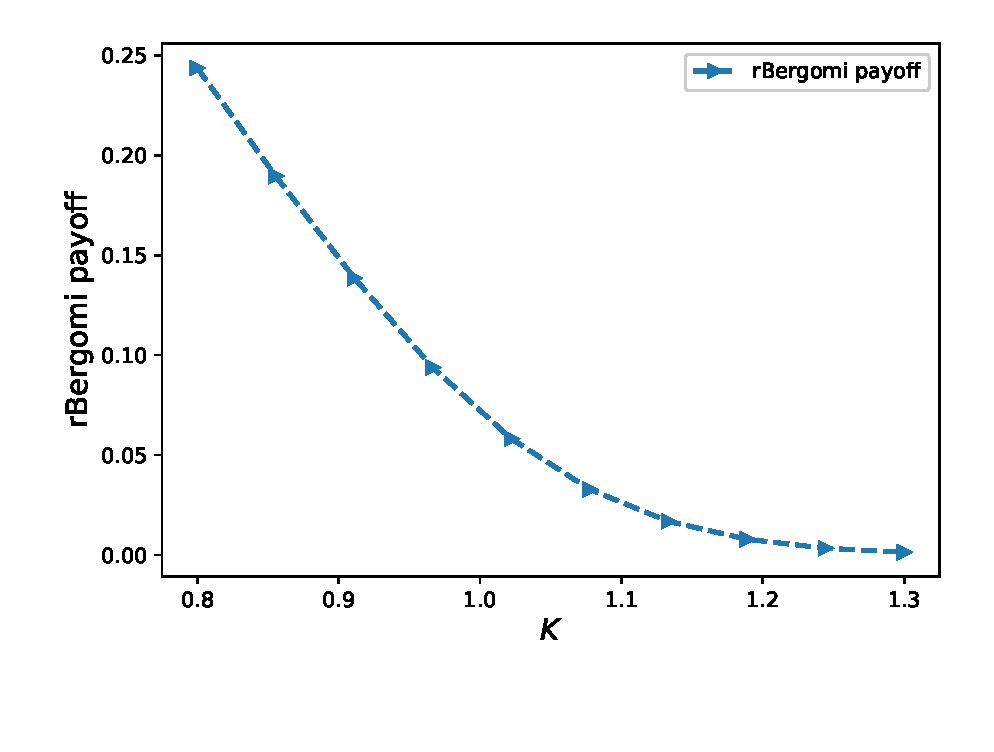
\includegraphics[width=0.95\linewidth]{./figures/payoff_plots_H_043/rBergomi_payoff_8steps_wrt_monyeness_2_H043}
		\caption{}
		\label{fig:rBergomi_payoff_4steps_wrt_monyeness_043_sub3}
	\end{subfigure}%
	\begin{subfigure}{.5\textwidth}
		\centering
		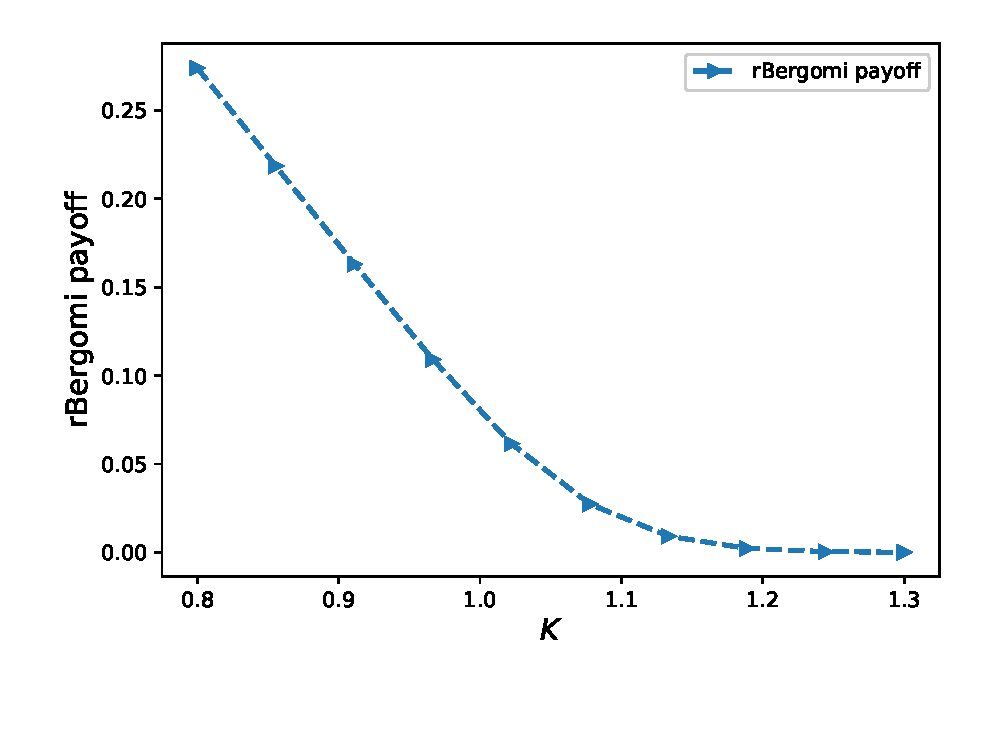
\includegraphics[width=0.95\linewidth]{./figures/payoff_plots_H_043/rBergomi_payoff_16steps_wrt_monyeness_2_H043}
		\caption{ }
		\label{fig:rBergomi_payoff_4steps_wrt_monyeness_043_sub4}
	\end{subfigure}%
	\caption{Black Scholes payoff for rBergomi model as a function of moneyness for $H=0.43$ a) $8$  time steps, b) $16$  time steps.}
	\label{fig:rBergomi_payoff_4steps_wrt_monyeness_H_043_2}
\end{figure}

\subsubsection*{Case $H=0.07$}

\begin{table}[h!]
	\centering
	\begin{tabular}{l*{6}{c}r}
		Method \textbackslash  Steps            & $2$ & $4$ & $8$ & $16$  \\
		\hline
		MISC ($TOl=10^{-1}$)  & $0.1064$ & $0.0899$ & $0.0733$ & $0.0956$  \\
		MISC ($TOl=10^{-2}$)  & $0.1226$ & $0.1022$ & $0.0933$ & $-$  \\
		MISC ($TOl=10^{-3}$)        & $0.1215$ &$0.1025$ &  $-$ &  $-$ \\
		MISC ($TOl=10^{-4}$)    & $0.1218$ & $0.0924$  & $-$ & $-$  \\
		%				MC method ($M=10^{6}$)    & $0.0840$ & $0.0781$  & $0.0746$ & $0.0729$  \\
		MC method ($M=10^{7}$)   & $\underset{(1.01e-04)}{0.0824} $  & $\underset{(4.63e-05)}{0.0783} $  & $\underset{ (3.95e-05)}{0.0776}$ & $\underset {(3.64e-05)}{0.0779} $  \\		
		\hline
	\end{tabular}
	\caption{ Call option price of the different methods for different number of time steps. Case $K=1$}
	\label{table: Call option price of the different methods for different number of time steps. Case $K=1$_H_007}
\end{table}

\begin{table}[h!]
	\centering
	\begin{tabular}{l*{6}{c}r}
		Method \textbackslash  Steps            & $2$ & $4$ & $8$ & $16$  \\
		\hline
		MISC ($TOl=10^{-1}$)  & $0.2156$ & $0.2002$ &  $0.2002$ &  $0.1910$  \\
		MISC ($TOl=10^{-2}$)  &  $0.2474$ &  $0.2378$ &  $0.2378$ & $-$  \\
		MISC ($TOl=10^{-3}$)        &  $0.2505$ & $0.2377$ &   $-$ &  $-$ \\
		MISC ($TOl=10^{-4}$)    &  $0.25$ &  $0.231$  & $-$ & $-$  \\
		%		MC method ($M=10^{6}$)    &  $0.6326$ &  $0.6332$  &  $0.6330$ &  $0.6337$  \\
		MC method ($M=10^{7}$)   & $\underset{(1.1e-04)}{0.2199} $   & $\underset{(6.03e-05)}{0.2212} $  & $\underset{(5.48e-05)}{0.2225}$ & $\underset{(5.27e-05)}{0.2233} $  \\			
		\hline
	\end{tabular}
	\caption{ Call option price of the different methods for different number of time steps. Case $K=0.8$}
	\label{table: Call option price of the different methods for different number of time steps. Case $K=0.8$_H_007}
\end{table}






\begin{table}[h!]
	\centering
	\begin{tabular}{l*{6}{c}r}
		Method \textbackslash  Steps            & $2$ & $4$ & $8$ & $16$  \\
		\hline
		MISC ($TOl=10^{-1}$)  & $0.0288$  & $0.0102$   & $0.0025$   &  $0.0005 $ \\
		MISC ($TOl=10^{-2}$)  & $0.0501$  & $0.0161$ &   $0.0025$  &   $0.0005$  \\
		MISC ($TOl=10^{-3}$)        &  $0.0515$ & $0.0335$  &  $-$  &   $-$ \\
		MISC ($TOl=10^{-4}$)    & $0.0525$   &  $-$   & $-$ & $-$  \\
		%		MC method ($M=10^{6}$)    &  $0.8646$  &   $0.8647$   &   $0.8643$  &   $0.8646$   \\
		MC method ($M=10^{7}$)   & $\underset{(9.57e-05)}{0.0207} $   & $\underset{(3.32e-05)}{0.0165} $  & $\underset{(2.43e-05)}{0.0144}$ & $\underset{(2e-05)}{0.0130} $  \\		
		\hline
	\end{tabular}
	\caption{ Call option price of the different methods for different number of time steps. Case $K=1.2$}
	\label{table: Call option price of the different methods for different number of time steps. Case $K=1.2$_H_007}
\end{table}




\begin{figure}[!h]
	\centering
	\begin{subfigure}{.5\textwidth}
		\centering
		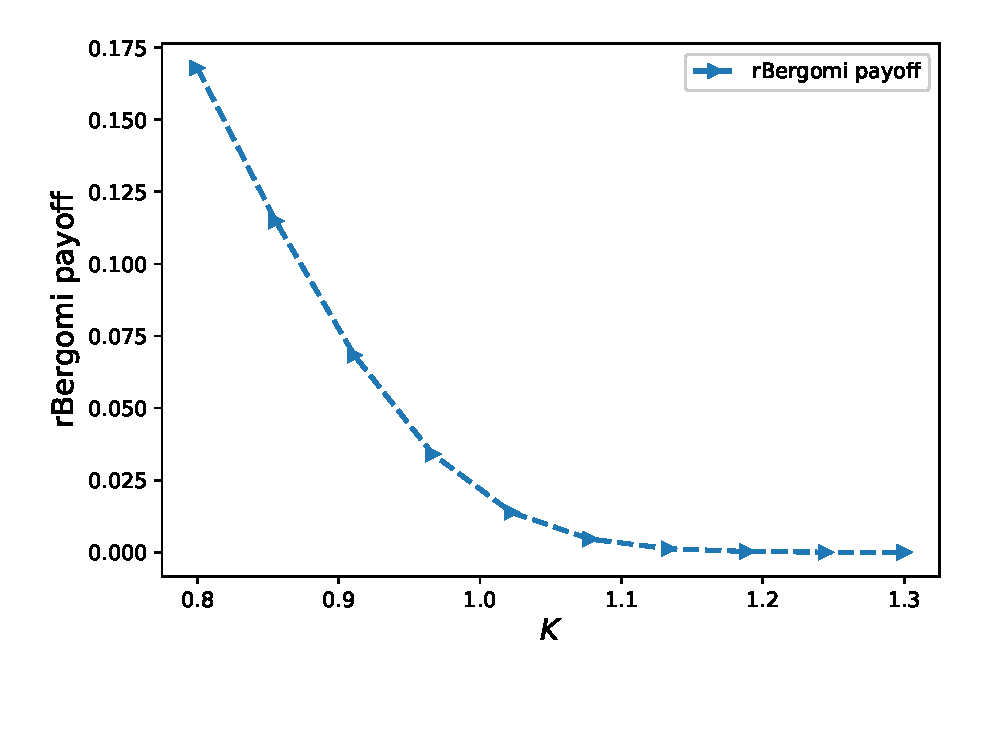
\includegraphics[width=0.95\linewidth]{./figures/payoff_plots_H_007/rBergomi_payoff_2steps_wrt_monyeness}
		\caption{}
		\label{fig:rBergomi_payoff_4steps_wrt_monyeness_sub1}
	\end{subfigure}%
	\begin{subfigure}{.5\textwidth}
		\centering
		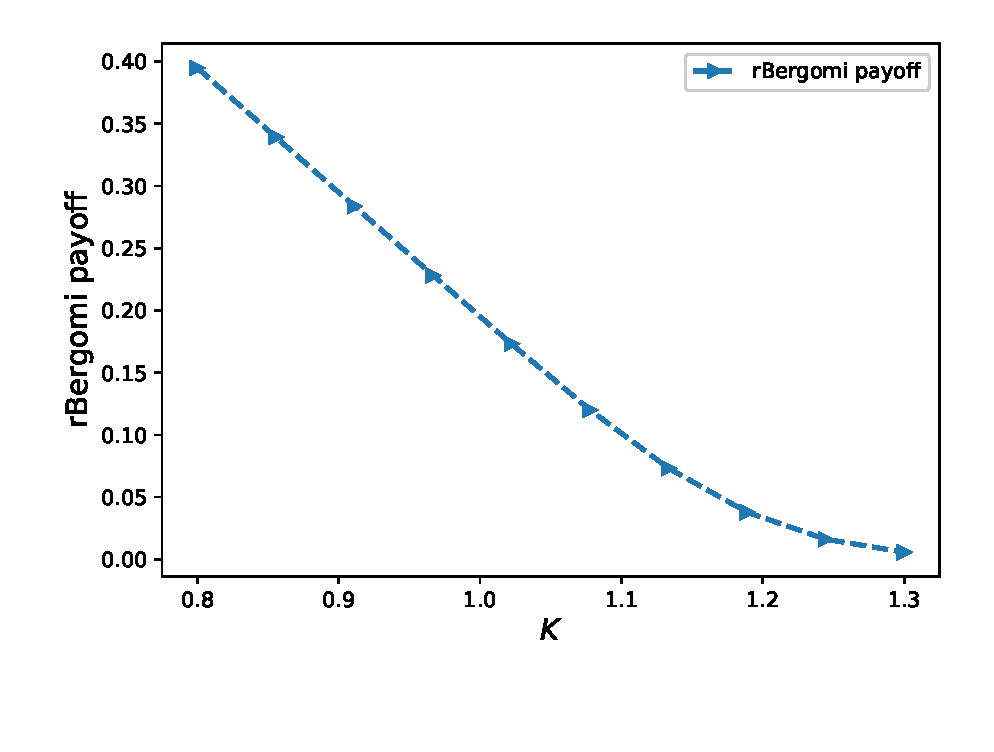
\includegraphics[width=0.95\linewidth]{./figures/payoff_plots_H_007/rBergomi_payoff_4steps_wrt_monyeness}
		\caption{ }
		\label{fig:rBergomi_payoff_4steps_wrt_monyeness_sub2}
	\end{subfigure}%
	\caption{Black Scholes payoff for rBergomi model as a function of moneyness a) $2$  time steps, b) $4$  time steps.}
	\label{fig:rBergomi_payoff_4steps_wrt_monyeness_1}
\end{figure}

\begin{figure}[!h]
	\centering
	\begin{subfigure}{.5\textwidth}
		\centering
		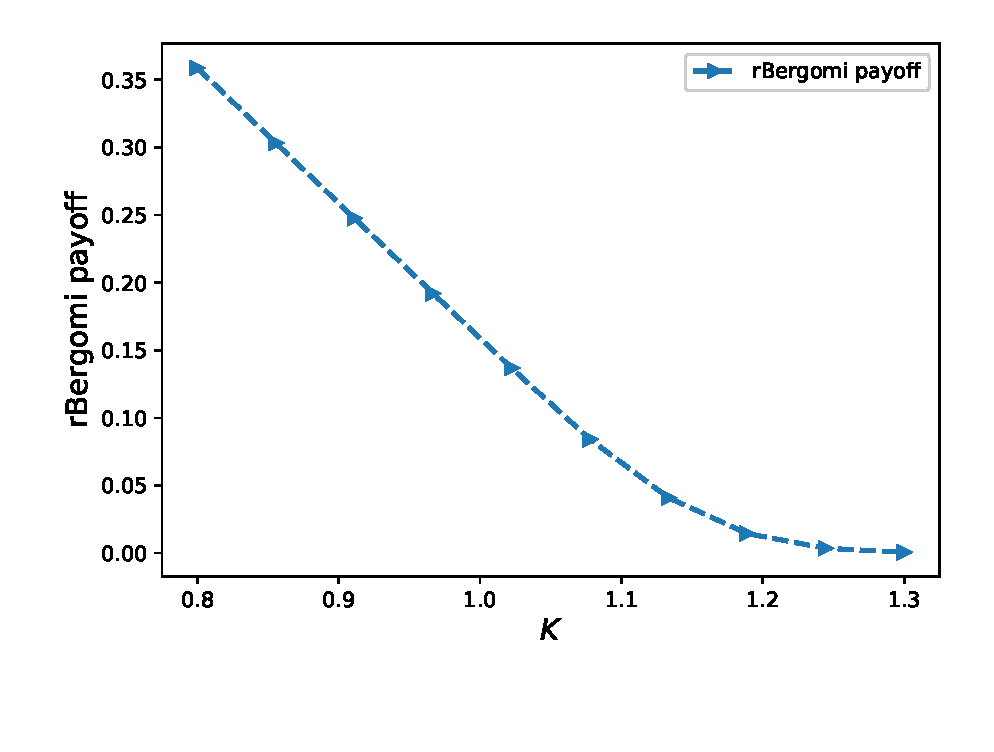
\includegraphics[width=0.95\linewidth]{./figures/payoff_plots_H_007/rBergomi_payoff_8steps_wrt_monyeness}
		\caption{}
		\label{fig:rBergomi_payoff_4steps_wrt_monyeness_sub3}
	\end{subfigure}%
	\begin{subfigure}{.5\textwidth}
		\centering
		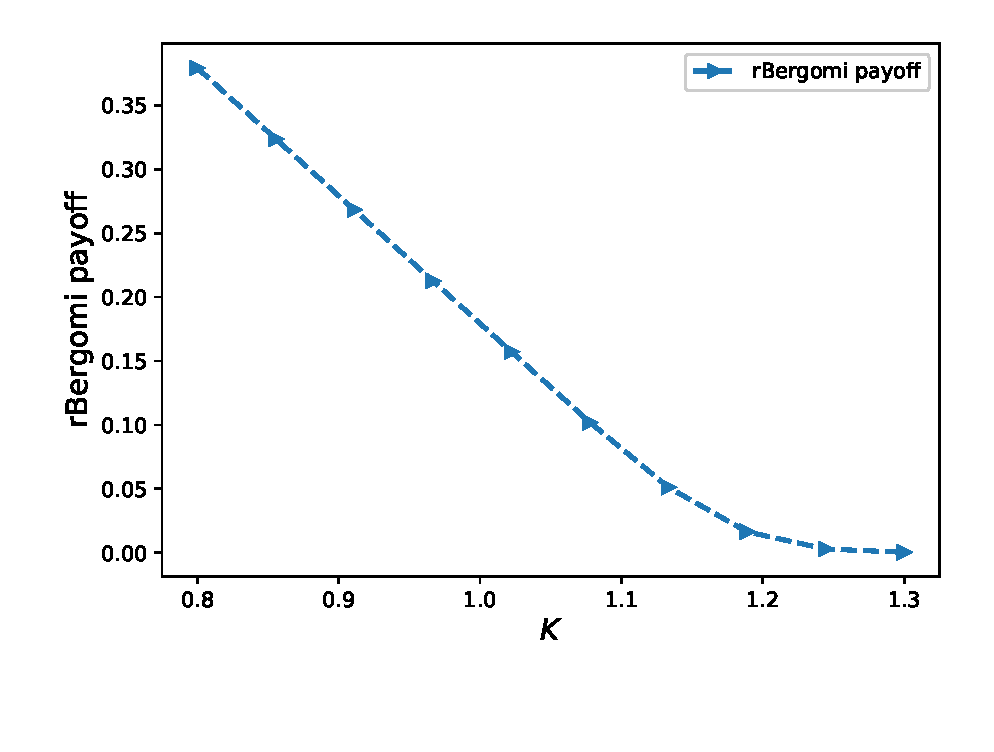
\includegraphics[width=0.95\linewidth]{./figures/payoff_plots_H_007/rBergomi_payoff_16steps_wrt_monyeness}
		\caption{ }
		\label{fig:rBergomi_payoff_4steps_wrt_monyeness_sub4}
	\end{subfigure}%
	\caption{Black Scholes payoff for rBergomi model as a function of moneyness a) $8$  time steps, b) $16$  time steps.}
	\label{fig:rBergomi_payoff_4steps_wrt_monyeness_2}
\end{figure}


\newpage
\subsection{Investigating mixed differences }\label{sec:mixed differences rbergomi}

\subsubsection*{Case $H=0.43$}
\subsubsection*{$N=8$ }
\begin{figure}[h!]
	\centering
	\begin{subfigure}{.5\textwidth}
		\centering
		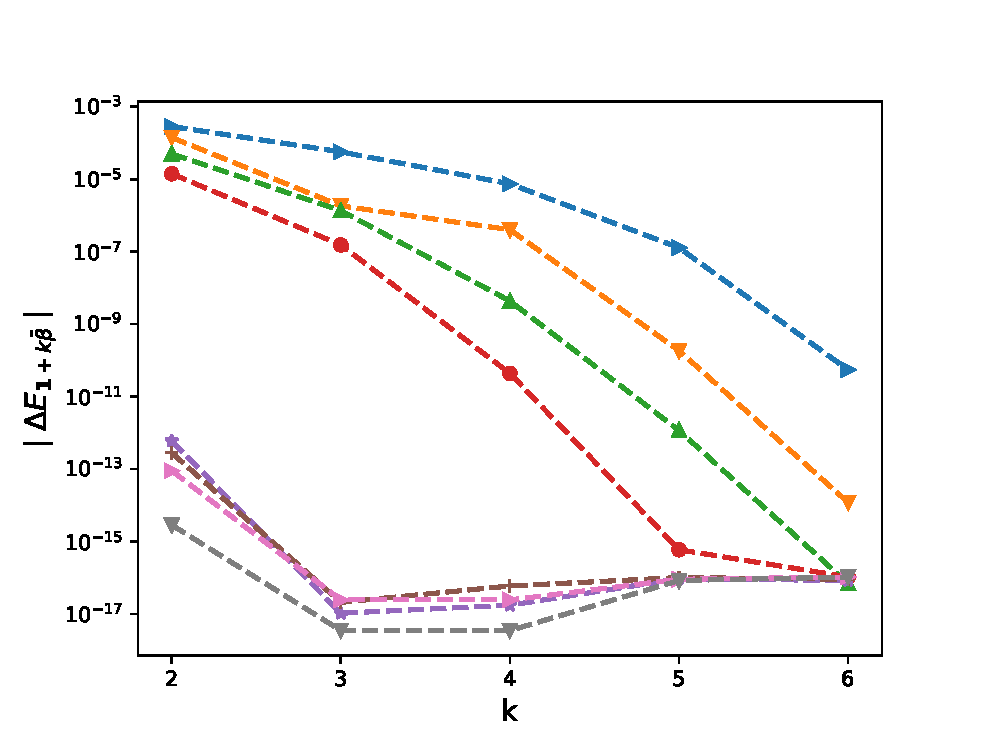
\includegraphics[width=1\linewidth]{./figures/mixed_diff_second_way/H_043/N_8/first_difference_rbergomi_8steps_H_043_K_1.eps}
		\caption{}
		\label{fig:sub3}
	\end{subfigure}%
	\begin{subfigure}{.5\textwidth}
		\centering
		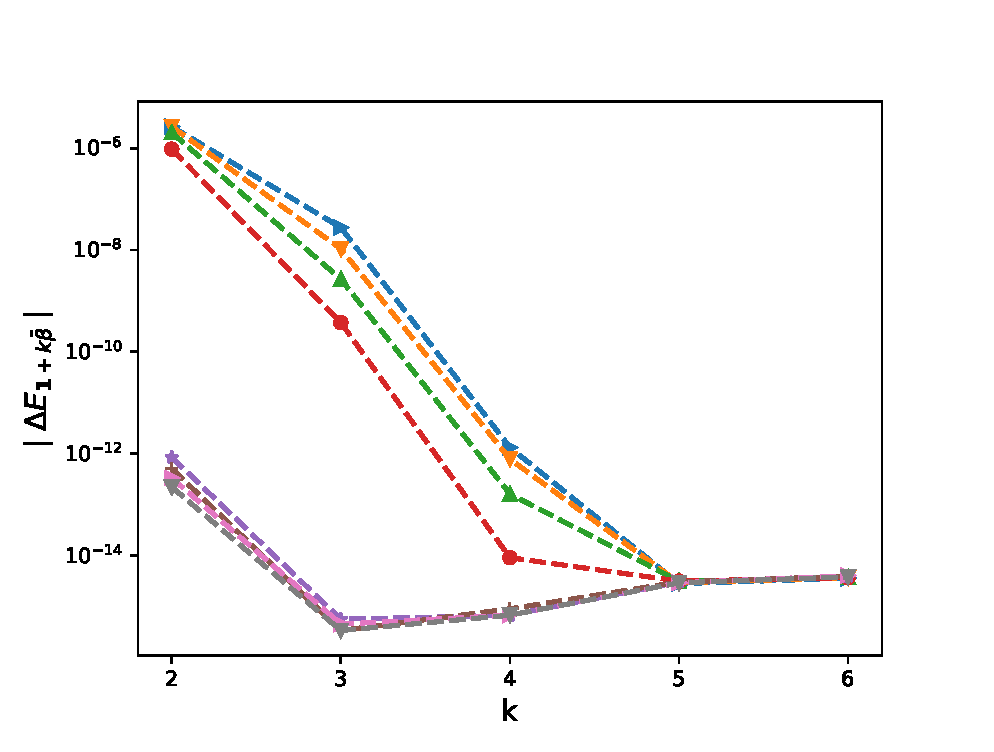
\includegraphics[width=1\linewidth]{./figures/mixed_diff_second_way/H_043/N_8/first_difference_rbergomi_8steps_H_043_K_exp__4.eps}
		\caption{}
		\label{fig:sub4}
	\end{subfigure}
	
	\caption{The rate of convergence of  first order differences $\abs{\Delta E_{\beta}}$ ($\beta=\mathbf{1}+k \bar{\beta}$)): a) $K=1$ b)  $K=\operatorname{exp}(-4).$}
	\label{fig:test2}
\end{figure}

\begin{figure}[h!]
	\centering
	\begin{subfigure}{.5\textwidth}
		\centering
		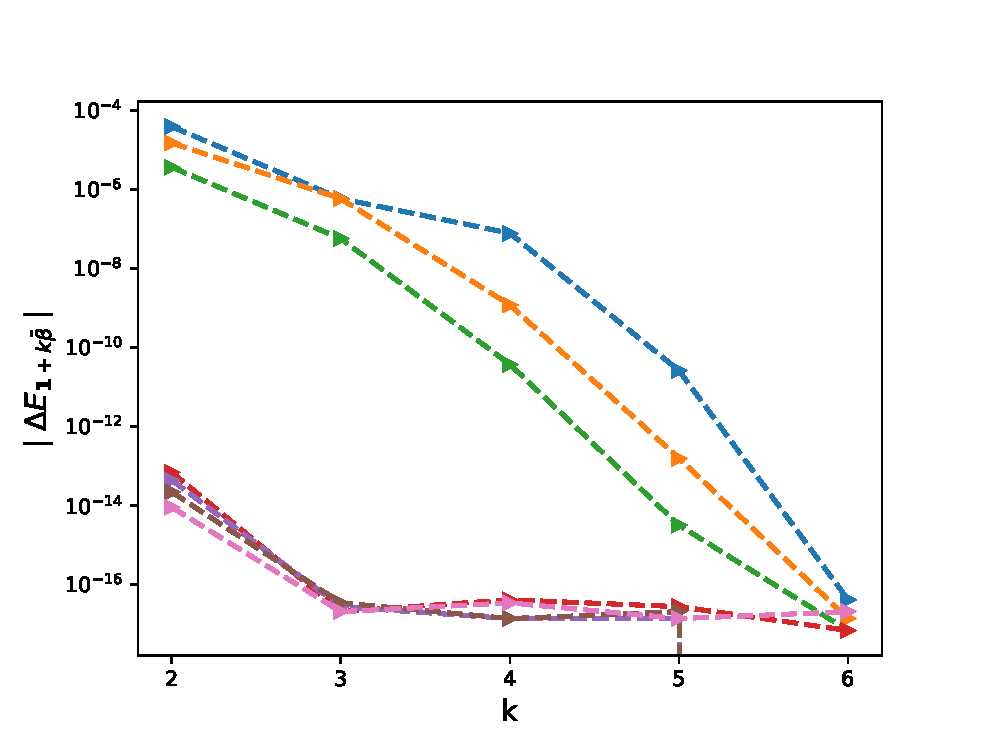
\includegraphics[width=1\linewidth]{./figures/mixed_diff_second_way/H_043/N_8/mixed_difference_order2_rbergomi_8steps_H_043_K_1.eps}
		\caption{}
		\label{fig:sub3}
	\end{subfigure}%
	\begin{subfigure}{.5\textwidth}
		\centering
		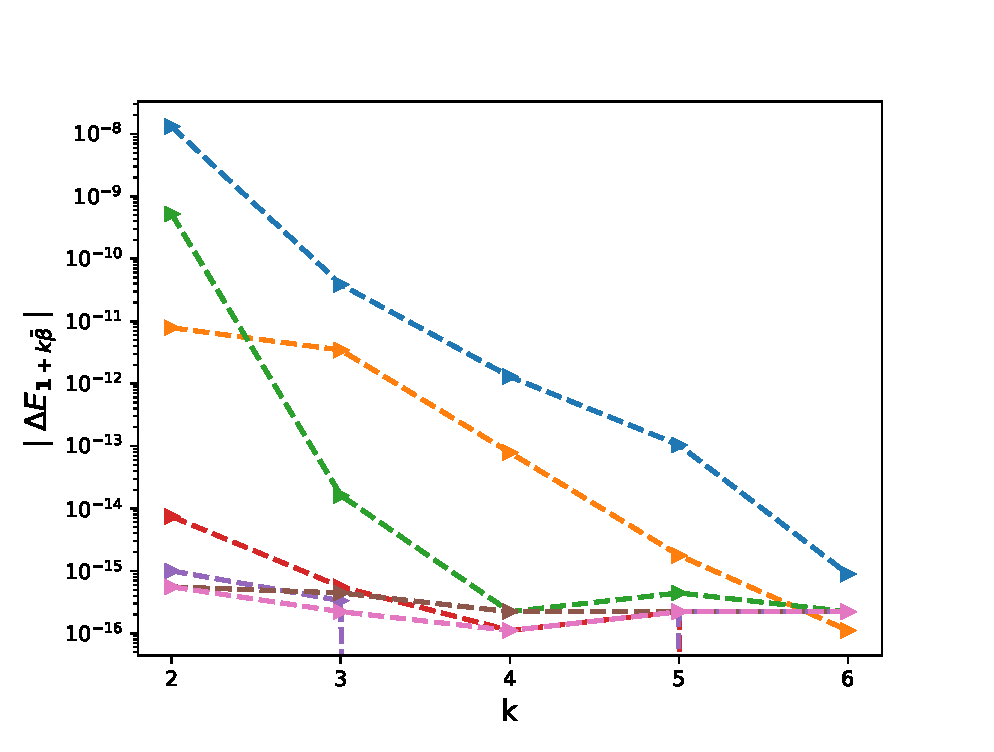
\includegraphics[width=1\linewidth]{./figures/mixed_diff_second_way/H_043/N_8/mixed_difference_order2_rbergomi_8steps_H_043_K_exp__4.eps}
		\caption{}
		\label{fig:sub4}
	\end{subfigure}
	
	\caption{The rate of convergence of  second order differences $\abs{\Delta E_{\beta}}$ ($\beta=\mathbf{1}+k \bar{\beta}$)): a) $K=1$ b)  $K=\operatorname{exp}(-4).$}
	\label{fig:test2}
\end{figure}

\newpage
\subsubsection*{$N=16$ }


\begin{figure}[h!]
	\centering
	\begin{subfigure}{.5\textwidth}
		\centering
		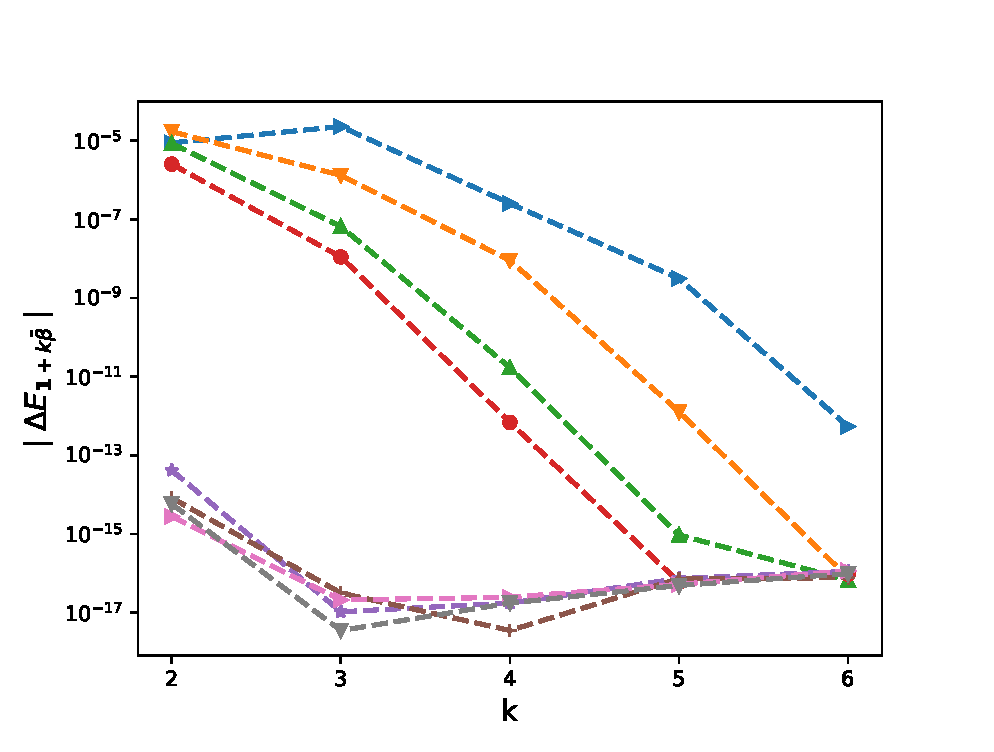
\includegraphics[width=1\linewidth]{./figures/mixed_diff_second_way/H_043/N_16/first_difference_rbergomi_16steps_H_043_K_1.eps}
		\caption{}
		\label{fig:sub3}
	\end{subfigure}%
	\begin{subfigure}{.5\textwidth}
		\centering
		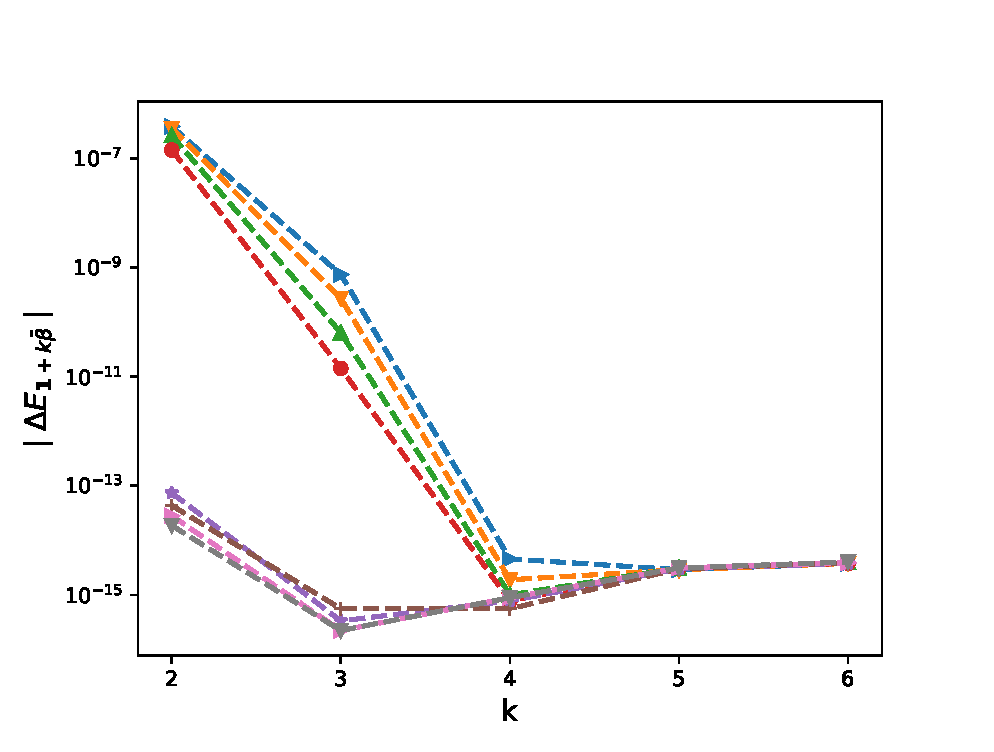
\includegraphics[width=1\linewidth]{./figures/mixed_diff_second_way/H_043/N_16/first_difference_rbergomi_16steps_H_043_K_exp__4.eps}
		\caption{}
		\label{fig:sub4}
	\end{subfigure}
	
	\caption{The rate of convergence of  first order differences $\abs{\Delta E_{\beta}}$ ($\beta=\mathbf{1}+k \bar{\beta}$)): a) $K=1$ b)  $K=\operatorname{exp}(-4).$}
	\label{fig:test2}
\end{figure}

\begin{figure}[h!]
	\centering
	\begin{subfigure}{.5\textwidth}
		\centering
		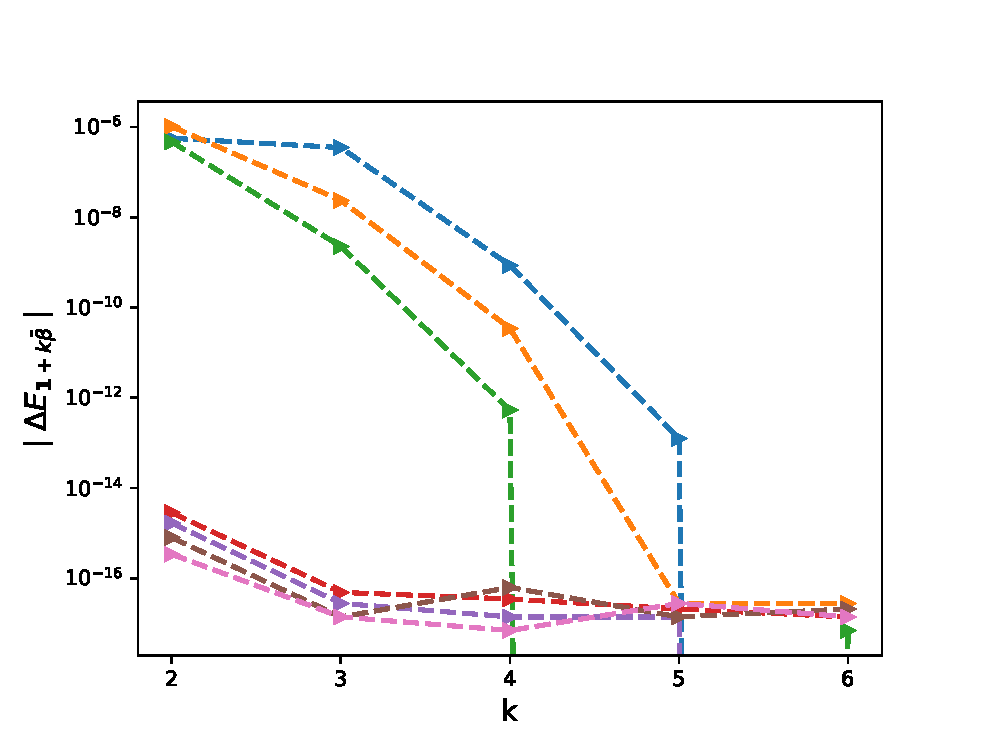
\includegraphics[width=1\linewidth]{./figures/mixed_diff_second_way/H_043/N_16/mixed_difference_order2_rbergomi_16steps_H_043_K_1.eps}
		\caption{}
		\label{fig:sub3}
	\end{subfigure}%
	\begin{subfigure}{.5\textwidth}
		\centering
		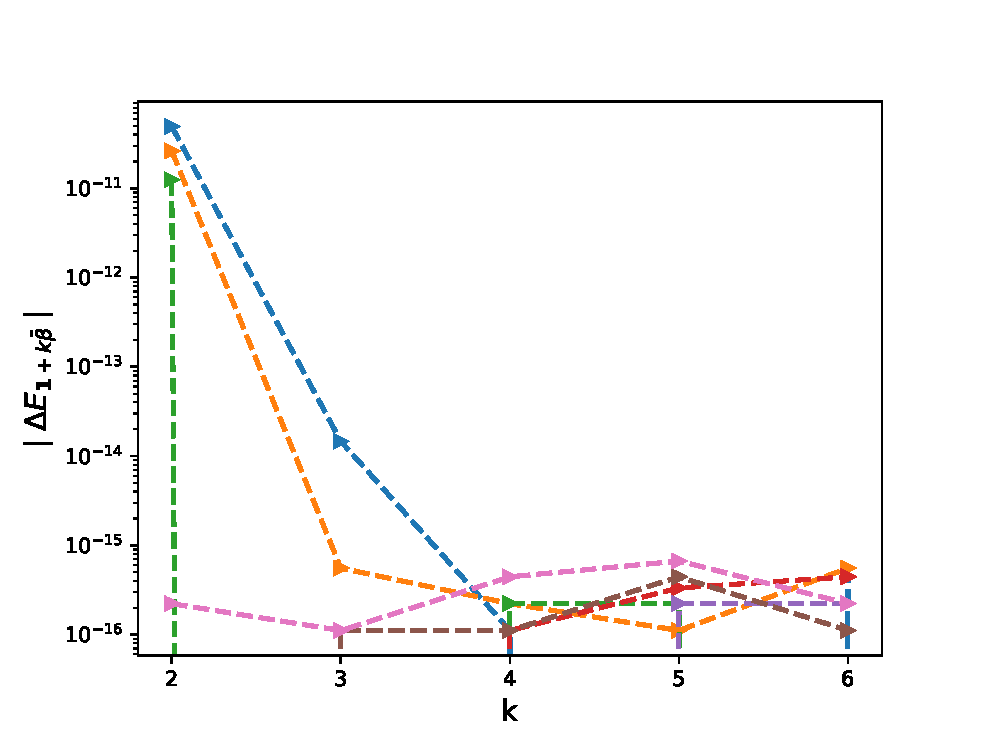
\includegraphics[width=1\linewidth]{./figures/mixed_diff_second_way/H_043/N_16/mixed_difference_order2_rbergomi_16steps_H_043_K_exp__4.eps}
		\caption{}
		\label{fig:sub4}
	\end{subfigure}
	
	\caption{The rate of convergence of  second order differences $\abs{\Delta E_{\beta}}$ ($\beta=\mathbf{1}+k \bar{\beta}$)): a) $K=1$ b)  $K=\operatorname{exp}(-4).$}
	\label{fig:test2}
\end{figure}



\newpage
\subsubsection*{Case $H=0.07$}
\subsubsection*{$N=8$ }

\begin{figure}[h!]
	\centering
	\begin{subfigure}{.5\textwidth}
		\centering
		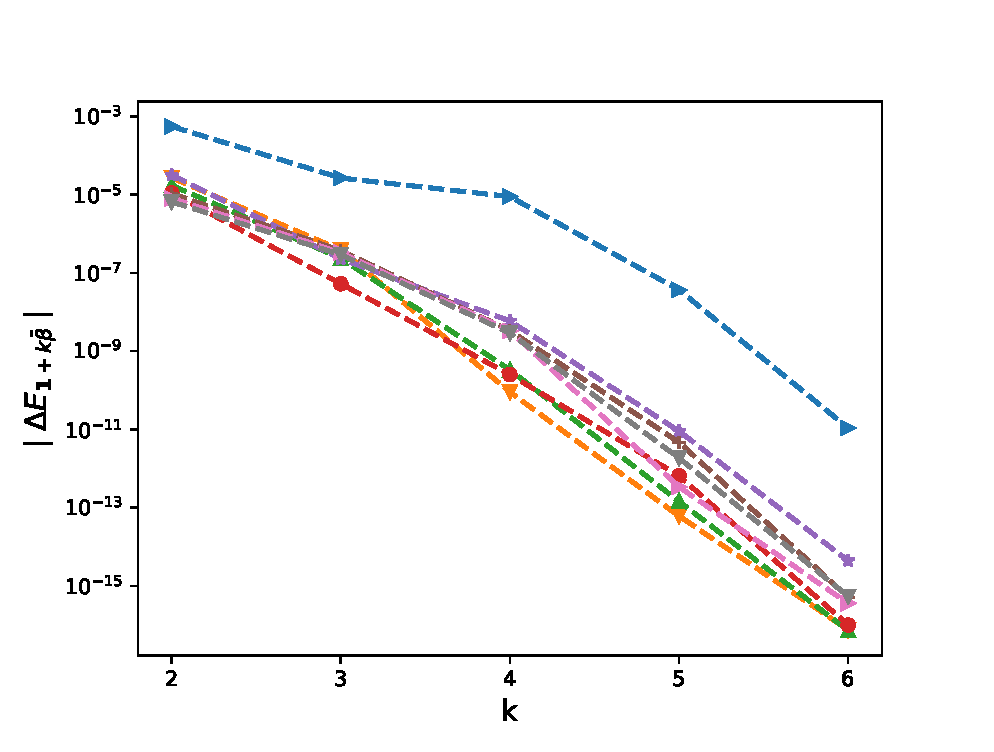
\includegraphics[width=1\linewidth]{./figures/mixed_diff_second_way/H_007/N_8/first_difference_rbergomi_8steps_H_007_K_1.eps}
		\caption{}
		\label{fig:sub3}
	\end{subfigure}%
	\begin{subfigure}{.5\textwidth}
		\centering
		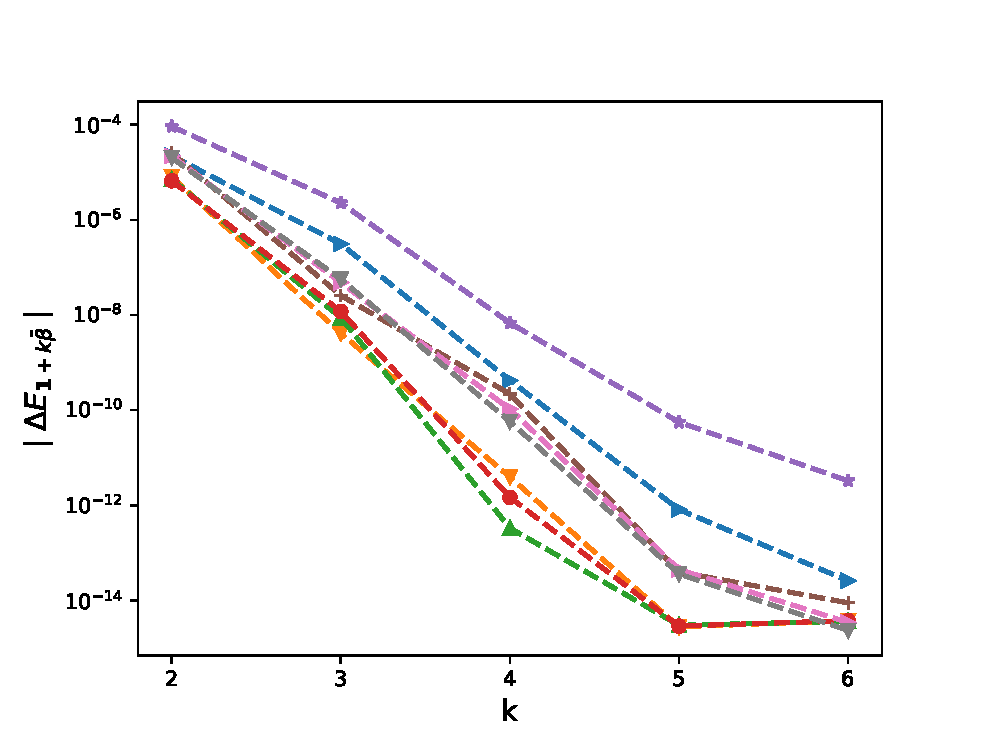
\includegraphics[width=1\linewidth]{./figures/mixed_diff_second_way/H_007/N_8/first_difference_rbergomi_8steps_H_007_K_exp__4.eps}
		\caption{}
		\label{fig:sub4}
	\end{subfigure}
	
	\caption{The rate of convergence of  first order differences $\abs{\Delta E_{\beta}}$ ($\beta=\mathbf{1}+k \bar{\beta}$)): a) $K=1$ b)  $K=\operatorname{exp}(-4).$}
	\label{fig:test2}
\end{figure}

\begin{figure}[h!]
	\centering
	\begin{subfigure}{.5\textwidth}
		\centering
		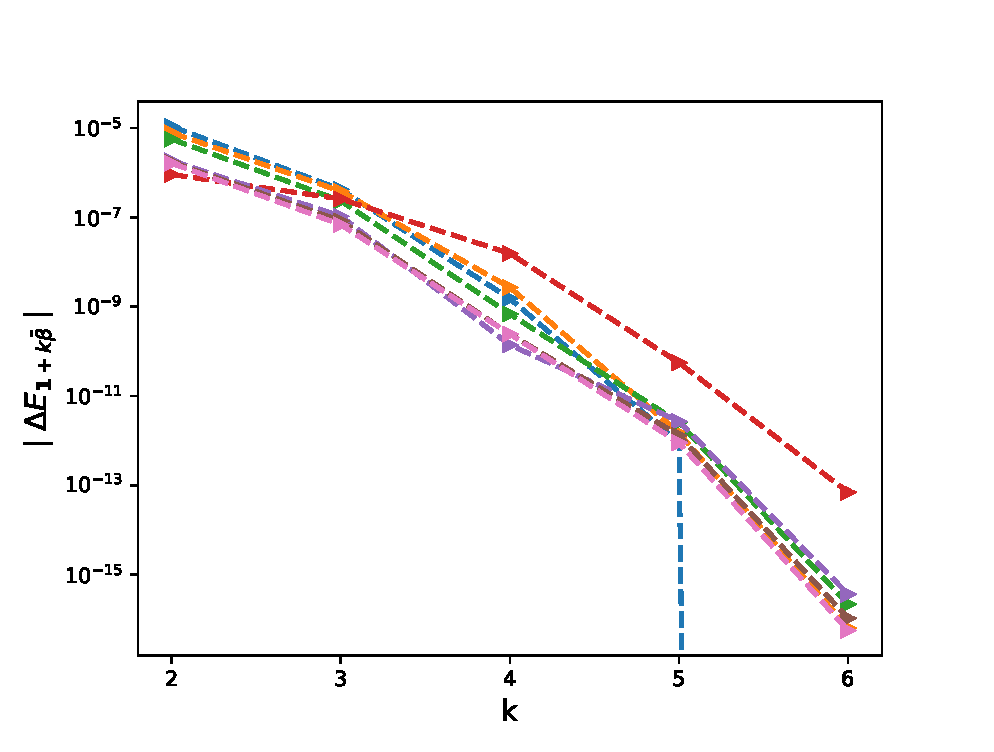
\includegraphics[width=1\linewidth]{./figures/mixed_diff_second_way/H_007/N_8/mixed_difference_order2_rbergomi_8steps_H_007_K_1.eps}
		\caption{}
		\label{fig:sub3}
	\end{subfigure}%
	\begin{subfigure}{.5\textwidth}
		\centering
		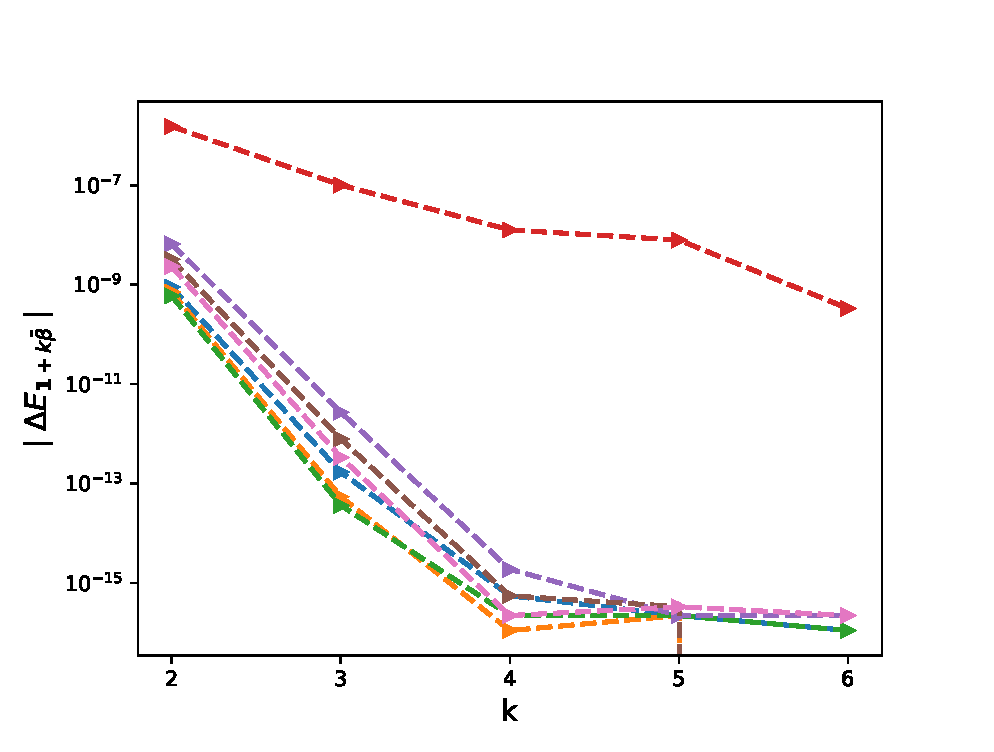
\includegraphics[width=1\linewidth]{./figures/mixed_diff_second_way/H_007/N_8/mixed_difference_order2_rbergomi_8steps_H_007_K_exp__4.eps}
		\caption{}
		\label{fig:sub4}
	\end{subfigure}
	
	\caption{The rate of convergence of  second order differences $\abs{\Delta E_{\beta}}$ ($\beta=\mathbf{1}+k \bar{\beta}$)): a) $K=1$ b)  $K=\operatorname{exp}(-4).$}
	\label{fig:test2}
\end{figure}


\newpage
\subsubsection*{$N=16$ }
\begin{figure}[h!]
	\centering
	\begin{subfigure}{.5\textwidth}
		\centering
		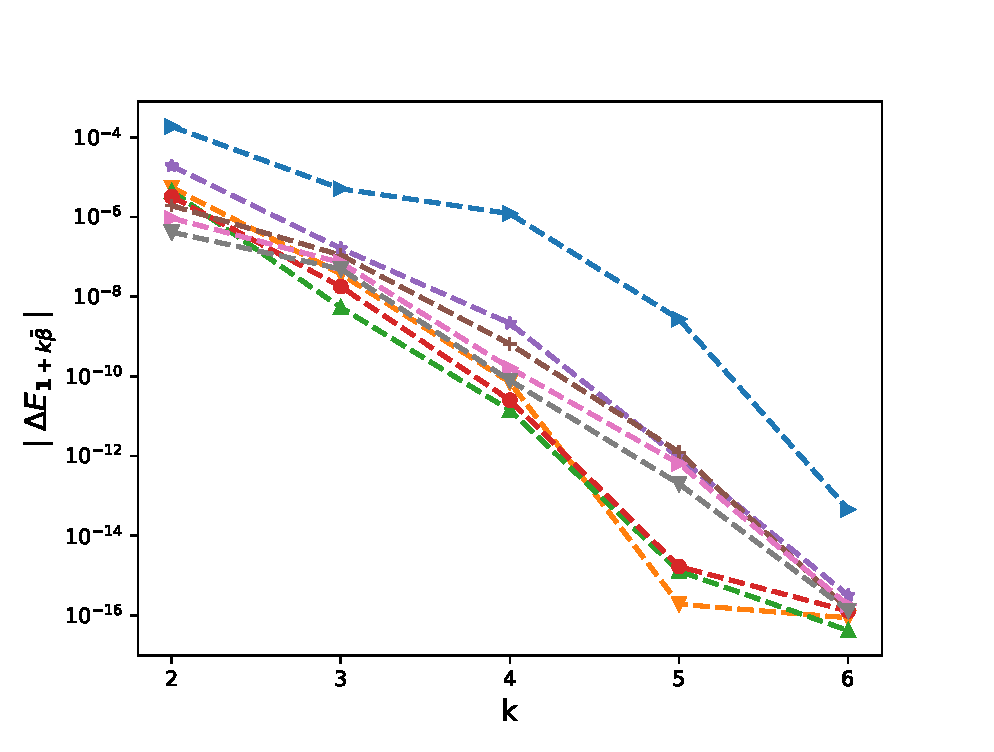
\includegraphics[width=1\linewidth]{./figures/mixed_diff_second_way/H_007/N_16/first_difference_rbergomi_16steps_H_007_K_1.eps}
		\caption{}
		\label{fig:sub3}
	\end{subfigure}%
	\begin{subfigure}{.5\textwidth}
		\centering
		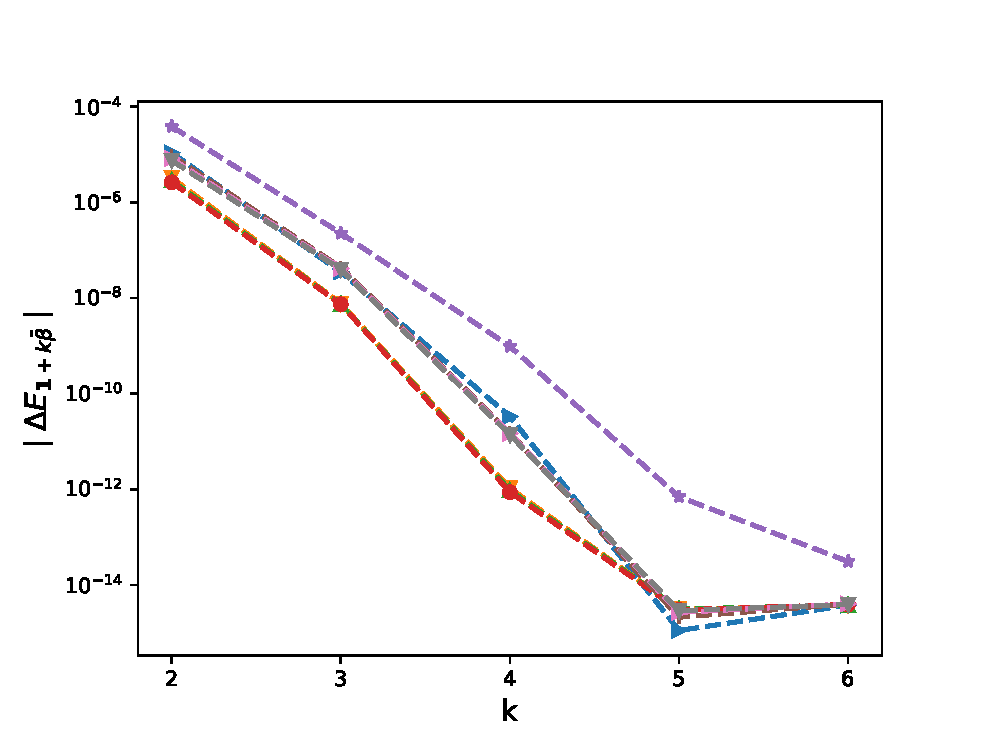
\includegraphics[width=1\linewidth]{./figures/mixed_diff_second_way/H_007/N_16/first_difference_rbergomi_16steps_H_007_K_exp__4.eps}
		\caption{}
		\label{fig:sub4}
	\end{subfigure}
	
	\caption{The rate of convergence of  first order differences $\abs{\Delta E_{\beta}}$ ($\beta=\mathbf{1}+k \bar{\beta}$)): a) $K=1$ b)  $K=\operatorname{exp}(-4).$}
	\label{fig:test2}
\end{figure}

\begin{figure}[h!]
	\centering
	\begin{subfigure}{.5\textwidth}
		\centering
		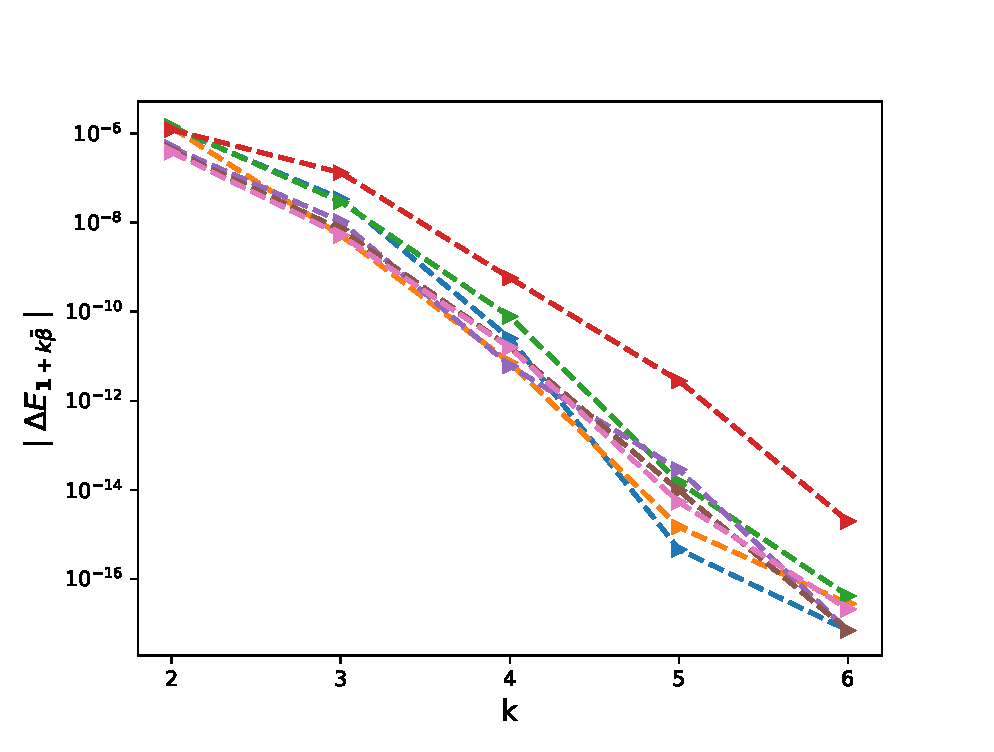
\includegraphics[width=1\linewidth]{./figures/mixed_diff_second_way/H_007/N_16/mixed_difference_order2_rbergomi_16steps_H_007_K_1.eps}
		\caption{}
		\label{fig:sub3}
	\end{subfigure}%
	\begin{subfigure}{.5\textwidth}
		\centering
		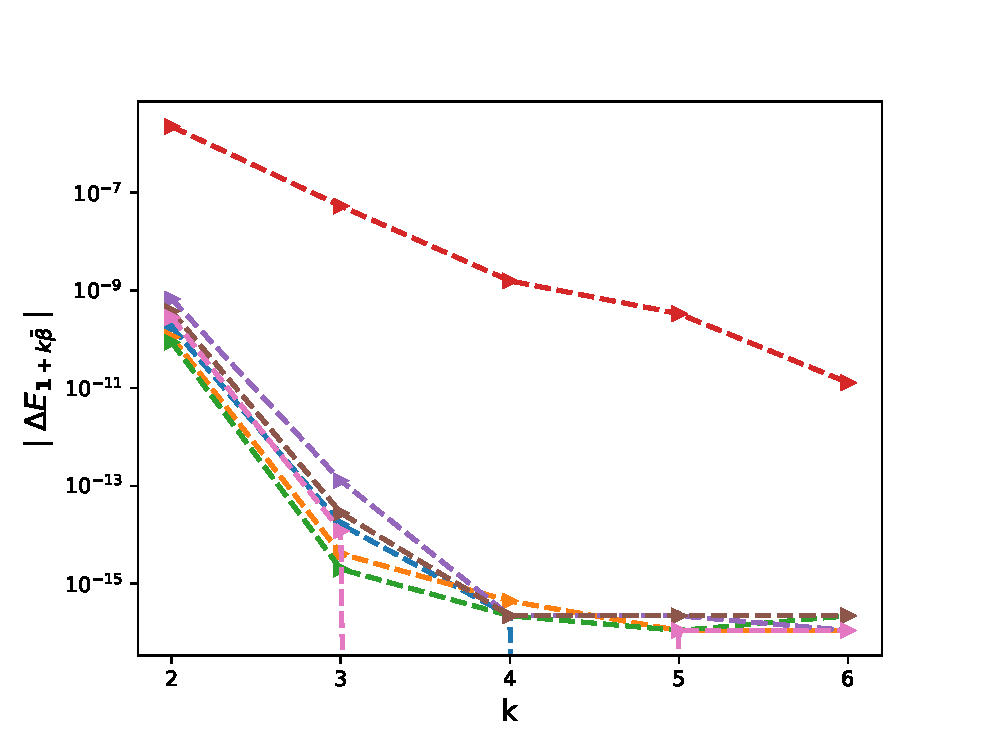
\includegraphics[width=1\linewidth]{./figures/mixed_diff_second_way/H_007/N_16/mixed_difference_order2_rbergomi_16steps_H_007_K_exp__4.eps}
		\caption{}
		\label{fig:sub4}
	\end{subfigure}
	
	\caption{The rate of convergence of  second order differences $\abs{\Delta E_{\beta}}$ ($\beta=\mathbf{1}+k \bar{\beta}$)): a) $K=1$ b)  $K=\operatorname{exp}(-4).$}
	\label{fig:test2}
\end{figure}


\newpage

\newpage
\subsection{Convergence plots using MISC ($H=0.43$)}\label{sec:Convergence plots using MISC_H_043}
\newpage
\subsubsection*{Case of $2$ time steps, $K=e^{-4}$}
\begin{figure}[!h]
	\centering
	\begin{subfigure}{.5\textwidth}
		\centering
		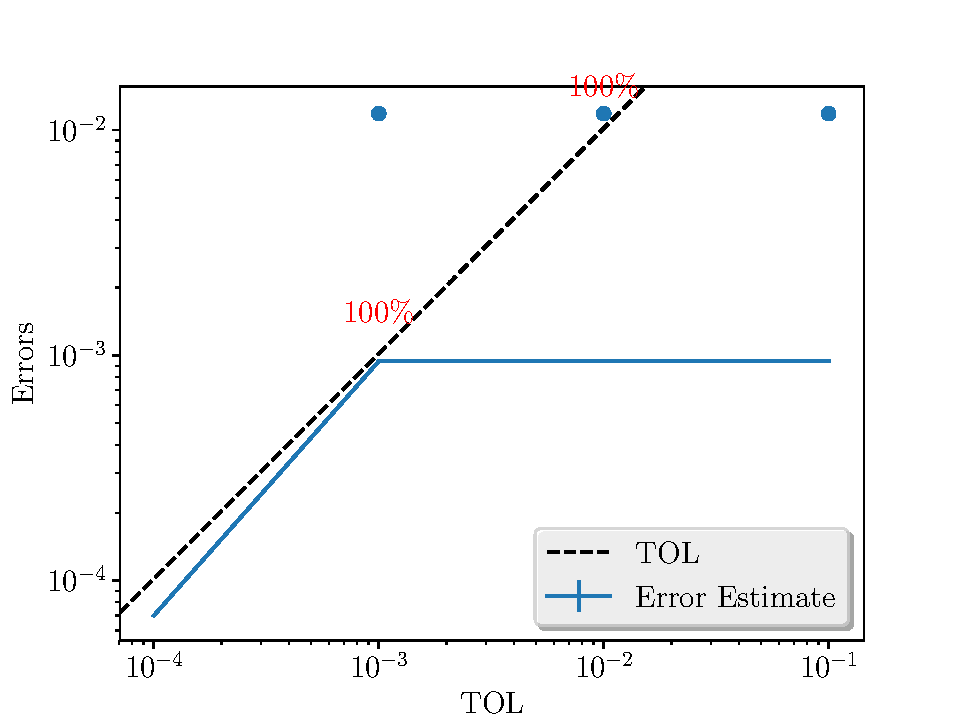
\includegraphics[width=1\linewidth]{./figures/rbergomi_2_steps_K_e__4/error_estimate.pdf}
		\caption{Error estimate}
		\label{fig:misc_rbergomi_2_steps_sub1}
	\end{subfigure}%
	\begin{subfigure}{.5\textwidth}
		\centering
		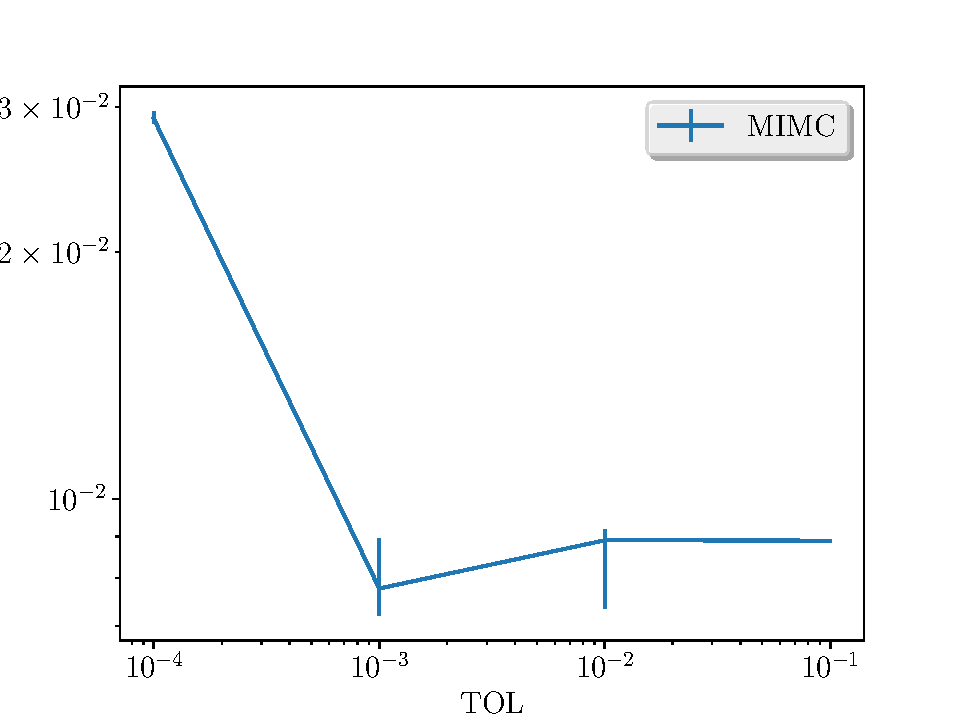
\includegraphics[width=1\linewidth]{./figures/rbergomi_2_steps_K_e__4/average_running_time.pdf}
		\caption{Average running time as a function of $TOL$}
		\label{fig:misc_rbergomi_2_steps_sub2}
	\end{subfigure}%
	\caption{Convergence and complexity results for the call payoff with rBergomi model.}
	\label{fig:misc_rbergomi_2_steps_1}
\end{figure}



\begin{figure}[!h]
	\centering
	\begin{subfigure}{.5\textwidth}
		\centering
		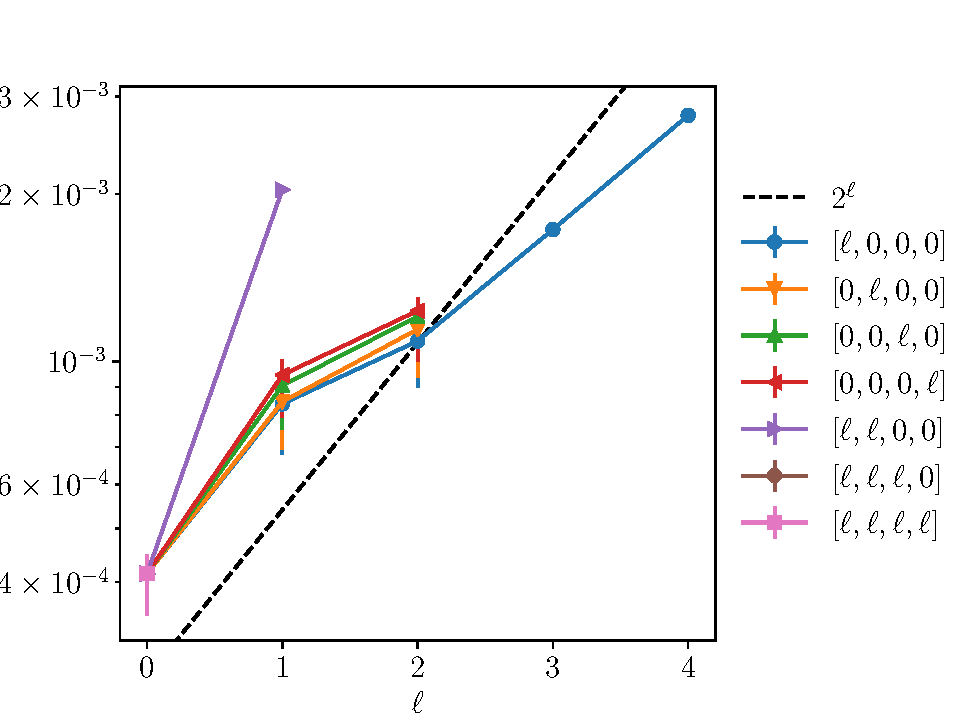
\includegraphics[width=0.95\linewidth]{./figures/rbergomi_2_steps_K_e__4/level_work.pdf}
		\caption{Average Computational time per level}
		\label{fig:misc_rbergomi_2_steps_sub3}
	\end{subfigure}%
	\begin{subfigure}{.5\textwidth}
		\centering
		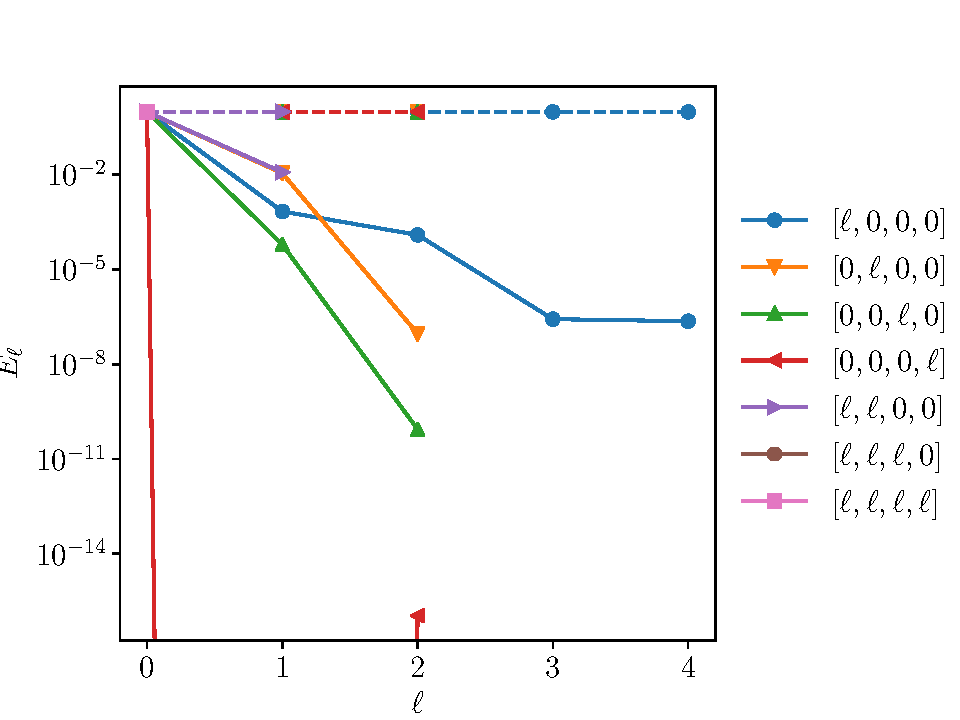
\includegraphics[width=0.95\linewidth]{./figures/rbergomi_2_steps_K_e__4/levels_error_rate.pdf}
		\caption{ The convergence rate of mixed differences per level}
		\label{fig:misc_rbergomi_2_steps_sub4}
	\end{subfigure}%
	\caption{Convergence and work rates for discretization levels  the call payoff with rBergomi model.}
	\label{fig:misc_rbergomi_2_steps_2}
\end{figure}
\newpage
\subsubsection*{Case of $2$ time steps, $K=1.2$}
\begin{figure}[!h]
	\centering
	\begin{subfigure}{.5\textwidth}
		\centering
		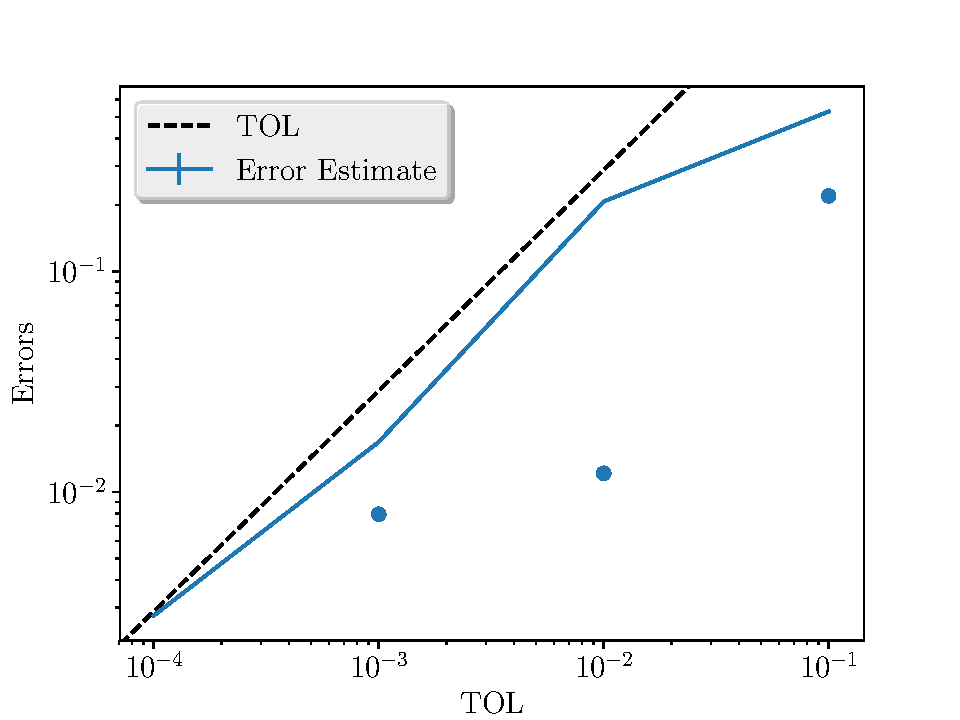
\includegraphics[width=1\linewidth]{./figures/rbergomi_2_steps_K_1_2/error_estimate.pdf}
		\caption{Error estimate}
		\label{fig:misc_rbergomi_2_steps_K_1_2_sub1}
	\end{subfigure}%
	\begin{subfigure}{.5\textwidth}
		\centering
		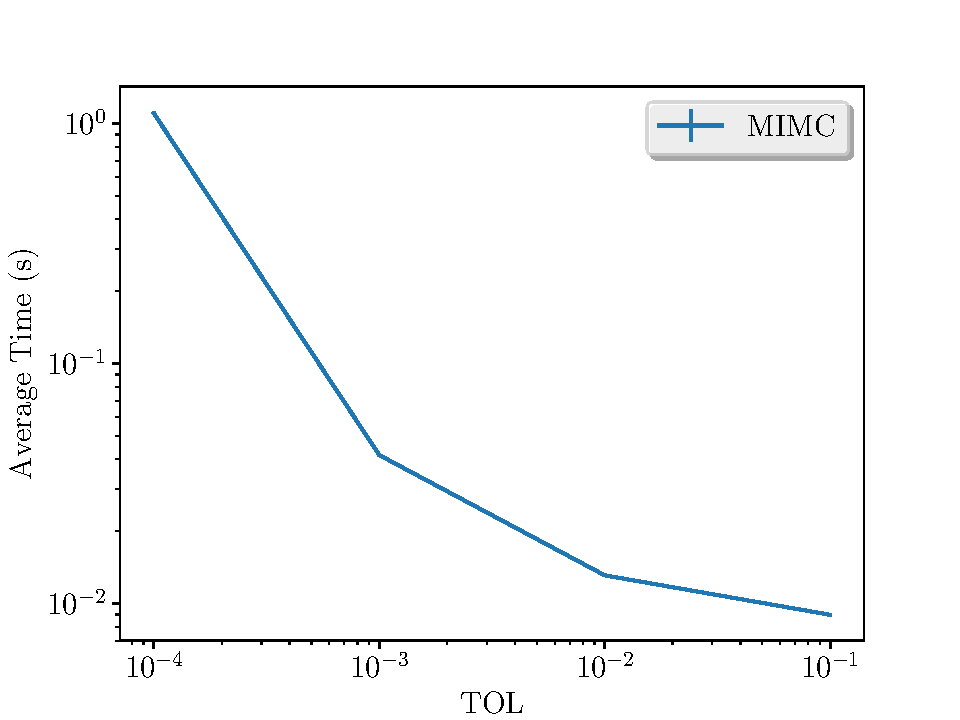
\includegraphics[width=1\linewidth]{./figures/rbergomi_2_steps_K_1_2/average_running_time.pdf}
		\caption{Average running time as a function of $TOL$}
		\label{fig:misc_rbergomi_2_steps_K_1_1_sub2}
	\end{subfigure}%
	\caption{Convergence and complexity results for the call payoff with rBergomi model.}
	\label{fig:misc_rbergomi_2_steps_K_1_2_1}
\end{figure}



\begin{figure}[!h]
	\centering
	\begin{subfigure}{.5\textwidth}
		\centering
		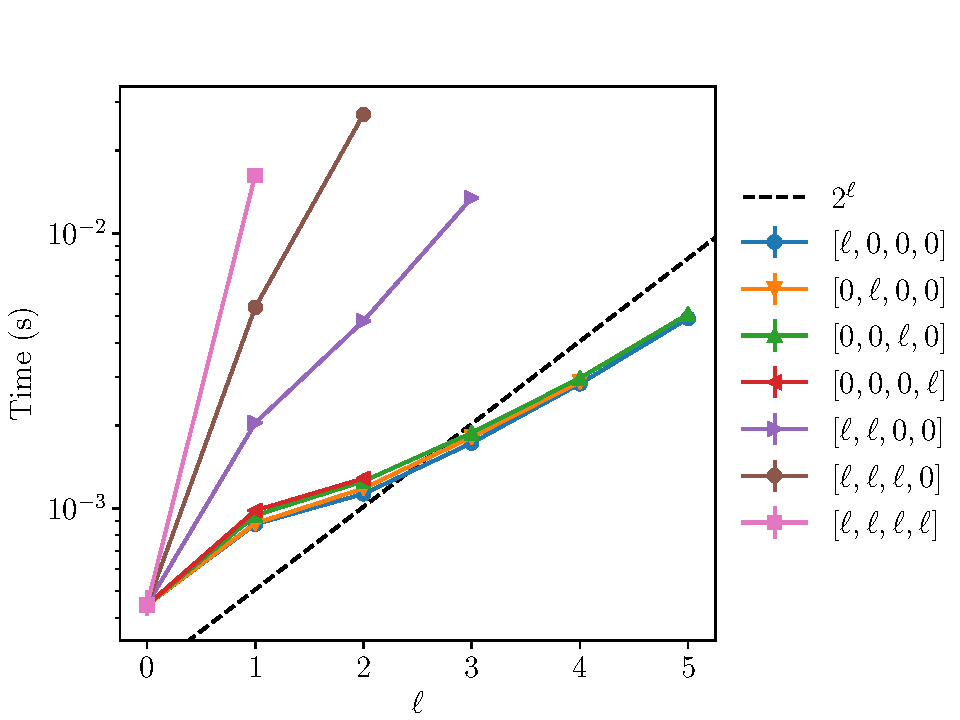
\includegraphics[width=0.95\linewidth]{./figures/rbergomi_2_steps_K_1_2/level_work.pdf}
		\caption{Average Computational time per level}
		\label{fig:misc_rbergomi_2_steps_K_1_2_sub3}
	\end{subfigure}%
	\begin{subfigure}{.5\textwidth}
		\centering
		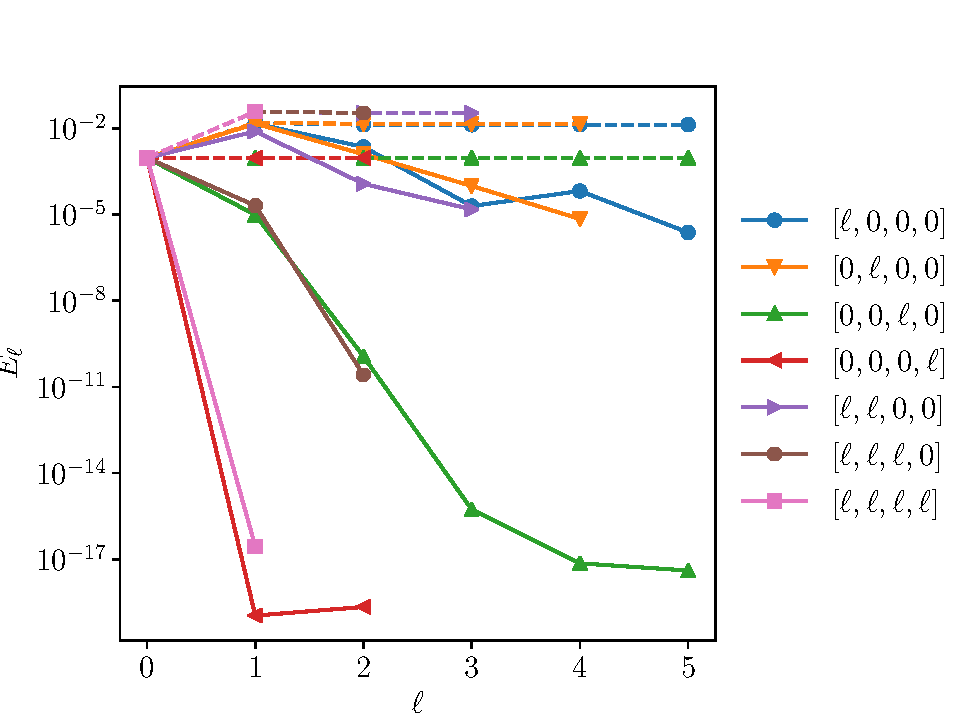
\includegraphics[width=0.95\linewidth]{./figures/rbergomi_2_steps_K_1_2/levels_error_rate.pdf}
		\caption{  The convergence rate of mixed differences per level}
		\label{fig:misc_rbergomi_2_steps_K_1_2_sub4}
	\end{subfigure}%
	\caption{Convergence and work rates for discretization levels  the call payoff with rBergomi model.}
	\label{fig:misc_rbergomi_2_steps_K_1_2_2}
\end{figure}


\newpage
\subsubsection*{Case of $4$ time steps, $K=e^{-4}$}
\begin{figure}[!h]
	\centering
	\begin{subfigure}{.5\textwidth}
		\centering
		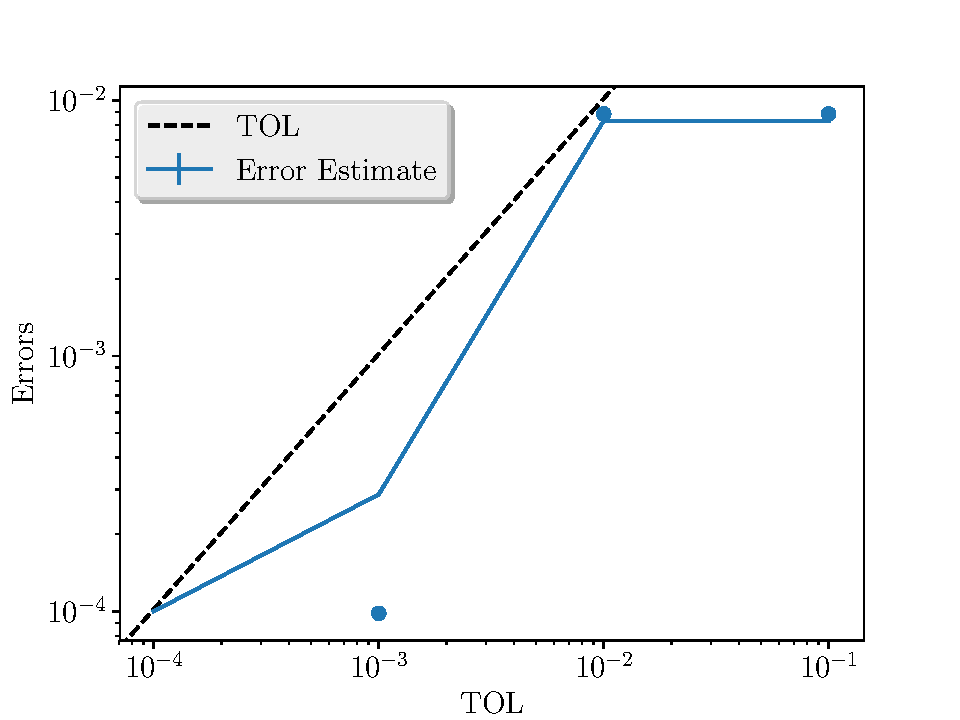
\includegraphics[width=1\linewidth]{./figures/rbergomi_4_steps_K_e__4/error_estimate.pdf}
		\caption{Error estimate}
		\label{fig:misc_rbergomi_4_steps_sub1}
	\end{subfigure}%
	\begin{subfigure}{.5\textwidth}
		\centering
		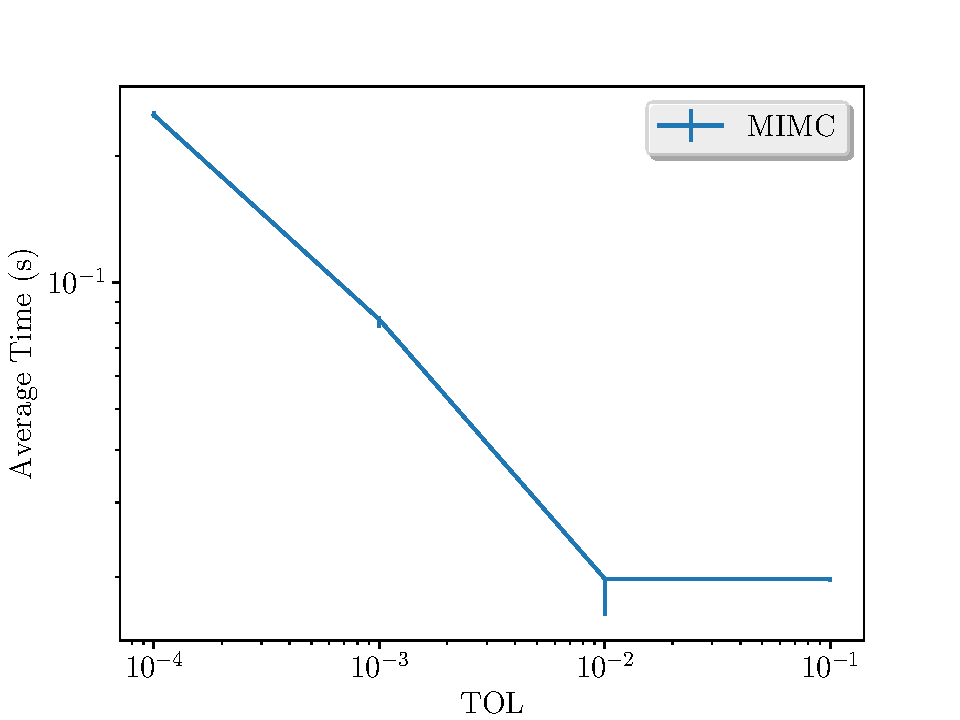
\includegraphics[width=1\linewidth]{./figures/rbergomi_4_steps_K_e__4/average_running_time.pdf}
		\caption{Average running time as a function of $TOL$}
		\label{fig:misc_rbergomi_4_steps_sub2}
	\end{subfigure}%
	\caption{Convergence and complexity results for the call payoff with rBergomi model.}
	\label{fig:misc_rbergomi_4_steps_1}
\end{figure}



\begin{figure}[!h]
	\centering
	\begin{subfigure}{.5\textwidth}
		\centering
		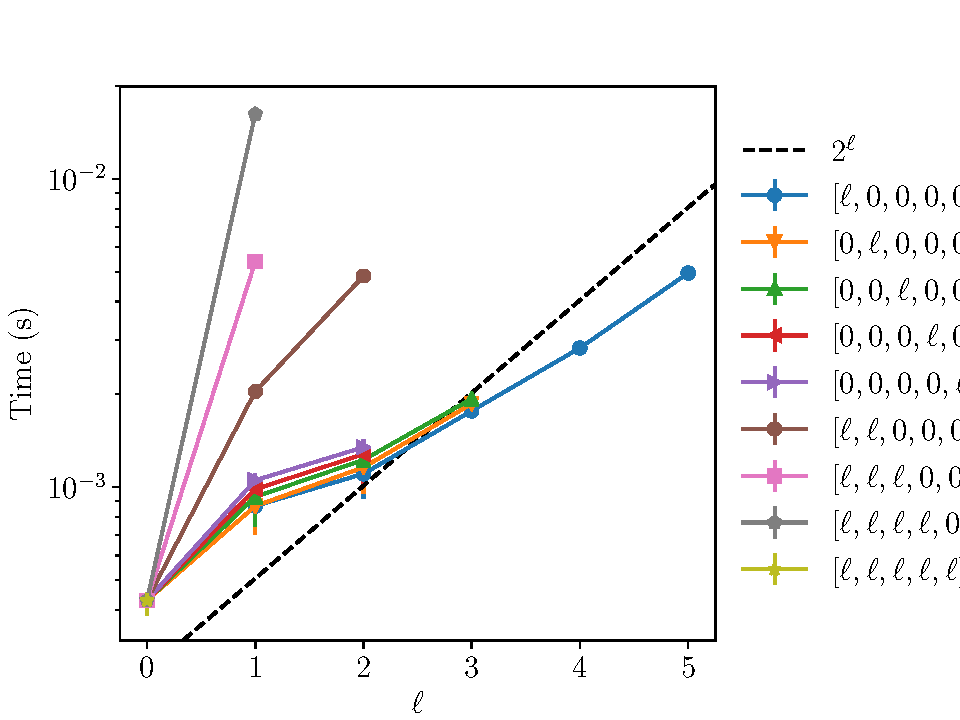
\includegraphics[width=0.95\linewidth]{./figures/rbergomi_4_steps_K_e__4/level_work.pdf}
		\caption{Average Computational time per level}
		\label{fig:misc_rbergomi_4_steps_sub3}
	\end{subfigure}%
	\begin{subfigure}{.5\textwidth}
		\centering
		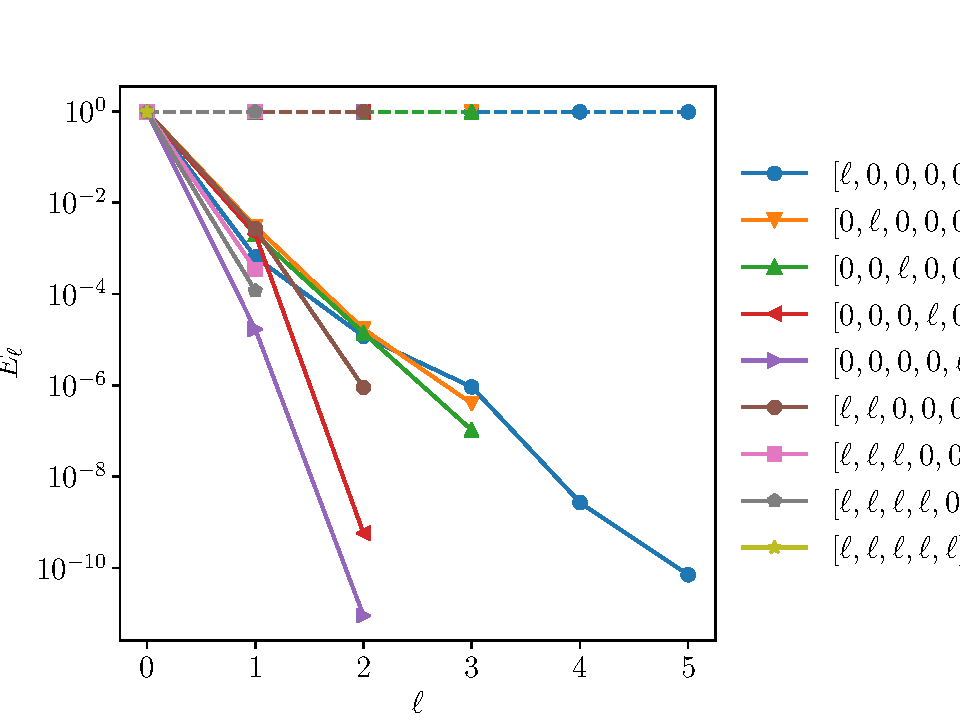
\includegraphics[width=0.95\linewidth]{./figures/rbergomi_4_steps_K_e__4/levels_error_rate.pdf}
		\caption{  The convergence rate of mixed differences per level}
		\label{fig:misc_rbergomi_4_steps_sub4}
	\end{subfigure}%
	\caption{Convergence and work rates for discretization levels  the call payoff with rBergomi model.}
	\label{fig:misc_rbergomi_4_steps_2}
\end{figure}
\newpage
\subsubsection*{Case of $4$ time steps, $K=1.2$}
\begin{figure}[!h]
	\centering
	\begin{subfigure}{.5\textwidth}
		\centering
		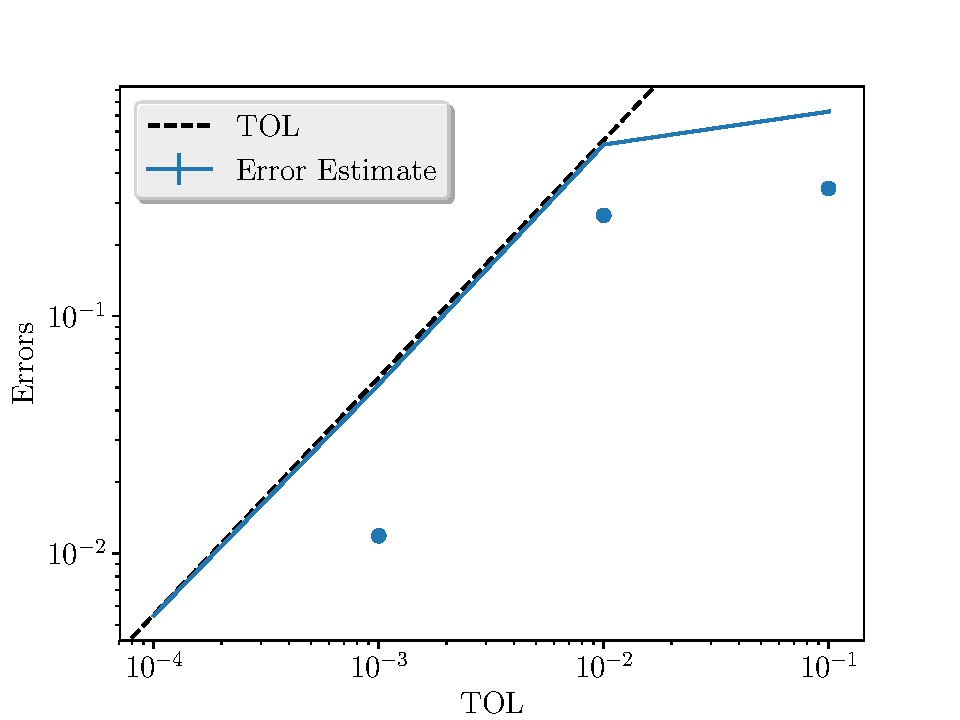
\includegraphics[width=1\linewidth]{./figures/rbergomi_4_steps_K_1_2/error_estimate.pdf}
		\caption{Error estimate}
		\label{fig:misc_rbergomi_4_steps_K_1_2_sub1}
	\end{subfigure}%
	\begin{subfigure}{.5\textwidth}
		\centering
		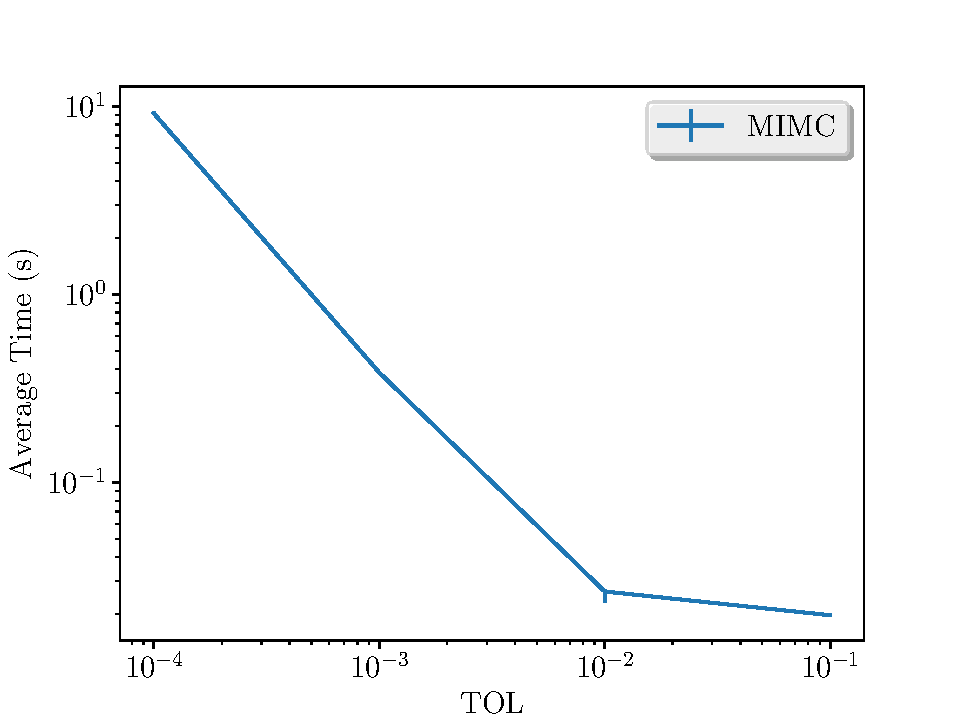
\includegraphics[width=1\linewidth]{./figures/rbergomi_4_steps_K_1_2/average_running_time.pdf}
		\caption{Average running time as a function of $TOL$}
		\label{fig:misc_rbergomi_4_steps_K_1_2_sub2}
	\end{subfigure}%
	\caption{Convergence and complexity results for the call payoff with rBergomi model.}
	\label{fig:misc_rbergomi_4_steps_K_1_2_1}
\end{figure}



\begin{figure}[!h]
	\centering
	\begin{subfigure}{.5\textwidth}
		\centering
		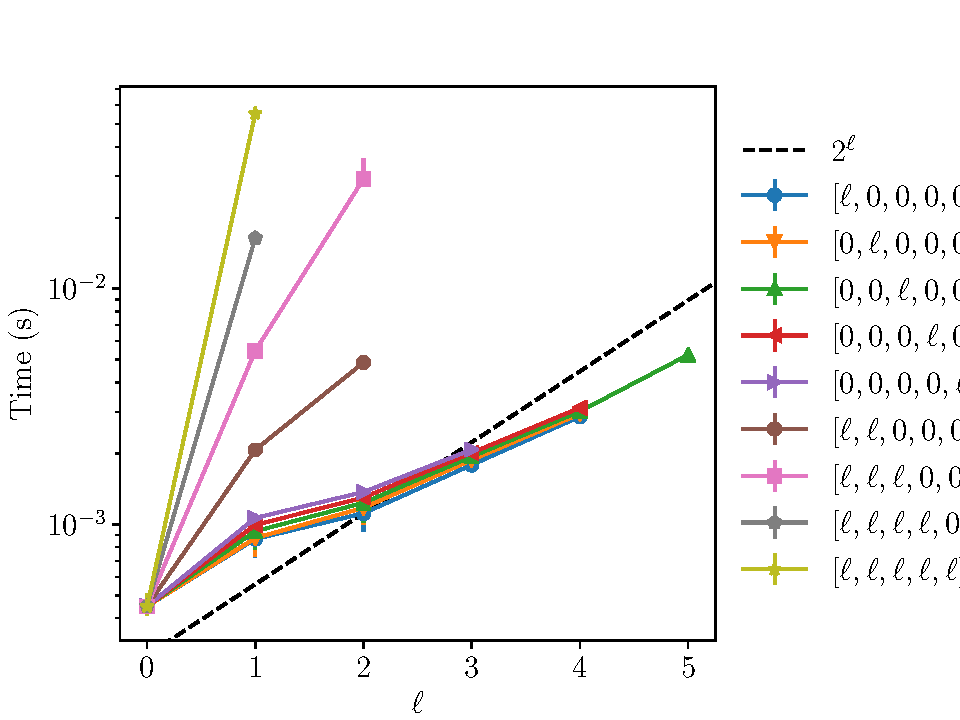
\includegraphics[width=0.95\linewidth]{./figures/rbergomi_4_steps_K_1_2/level_work.pdf}
		\caption{Average Computational time per level}
		\label{fig:misc_rbergomi_4_steps_K_2_sub3}
	\end{subfigure}%
	\begin{subfigure}{.5\textwidth}
		\centering
		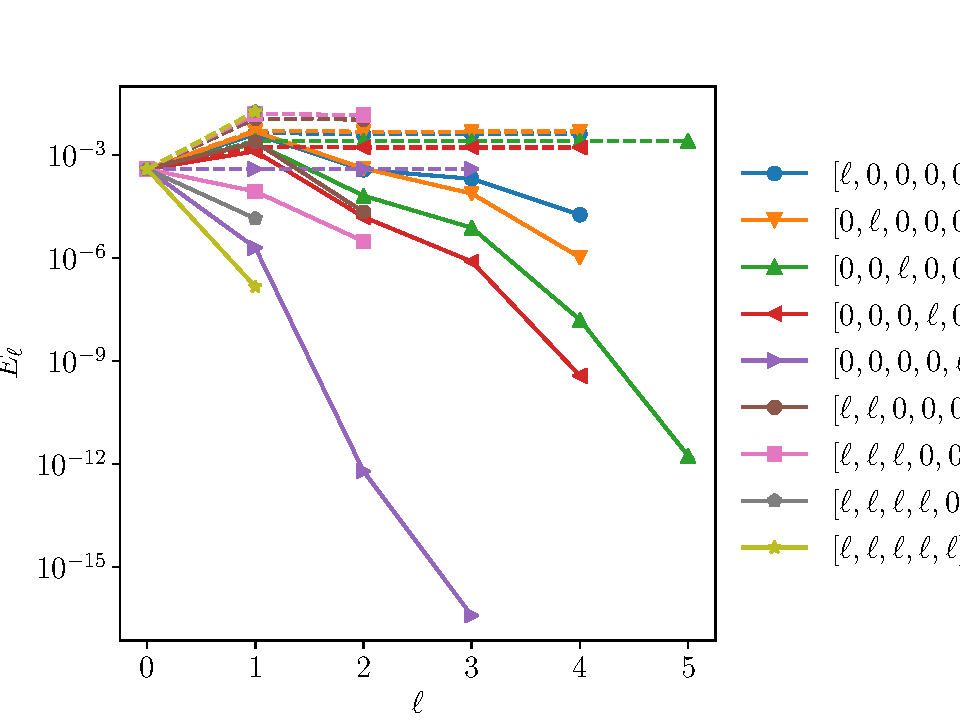
\includegraphics[width=0.95\linewidth]{./figures/rbergomi_4_steps_K_1_2/levels_error_rate.pdf}
		\caption{  The convergence rate of mixed differences per level}
		\label{fig:misc_rbergomi_4_steps_K_1_2_sub4}
	\end{subfigure}%
	\caption{Convergence and work rates for discretization levels  the call payoff with rBergomi model.}
	\label{fig:misc_rbergomi_4_steps_K_1_2_2}
\end{figure}



\newpage
\subsubsection*{Case of $8$ time steps, $K=e^{-4}$}
\begin{figure}[!h]
	\centering
	\begin{subfigure}{.5\textwidth}
		\centering
		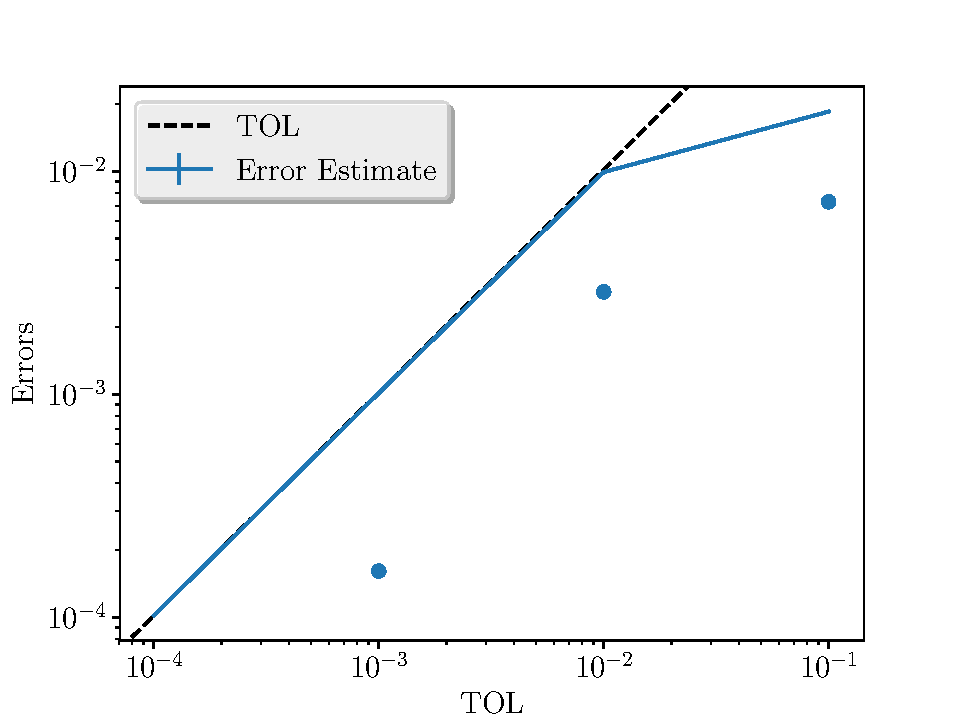
\includegraphics[width=1\linewidth]{./figures/rbergomi_8_steps_K_e__4/error_estimate.pdf}
		\caption{Error estimate}
		\label{fig:misc_rbergomi_8_steps_sub1}
	\end{subfigure}%
	\begin{subfigure}{.5\textwidth}
		\centering
		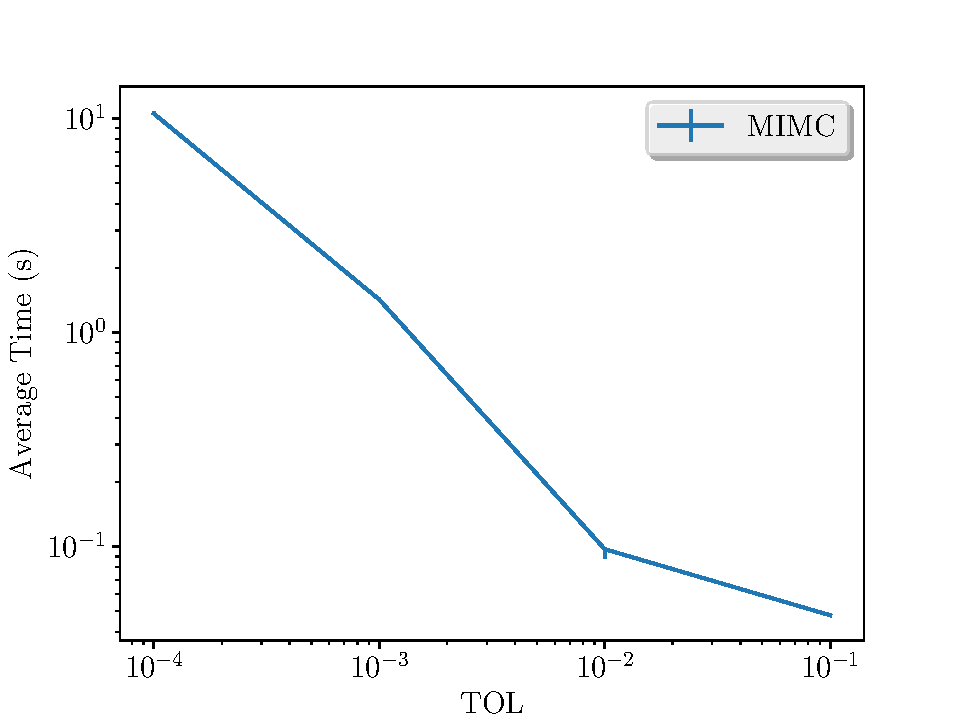
\includegraphics[width=1\linewidth]{./figures/rbergomi_8_steps_K_e__4/average_running_time.pdf}
		\caption{Average running time as a function of $TOL$}
		\label{fig:misc_rbergomi_8_steps_sub2}
	\end{subfigure}%
	\caption{Convergence and complexity results for the call payoff with rBergomi model.}
	\label{fig:misc_rbergomi_8_steps_1}
\end{figure}



\begin{figure}[!h]
	\centering
	\begin{subfigure}{.5\textwidth}
		\centering
		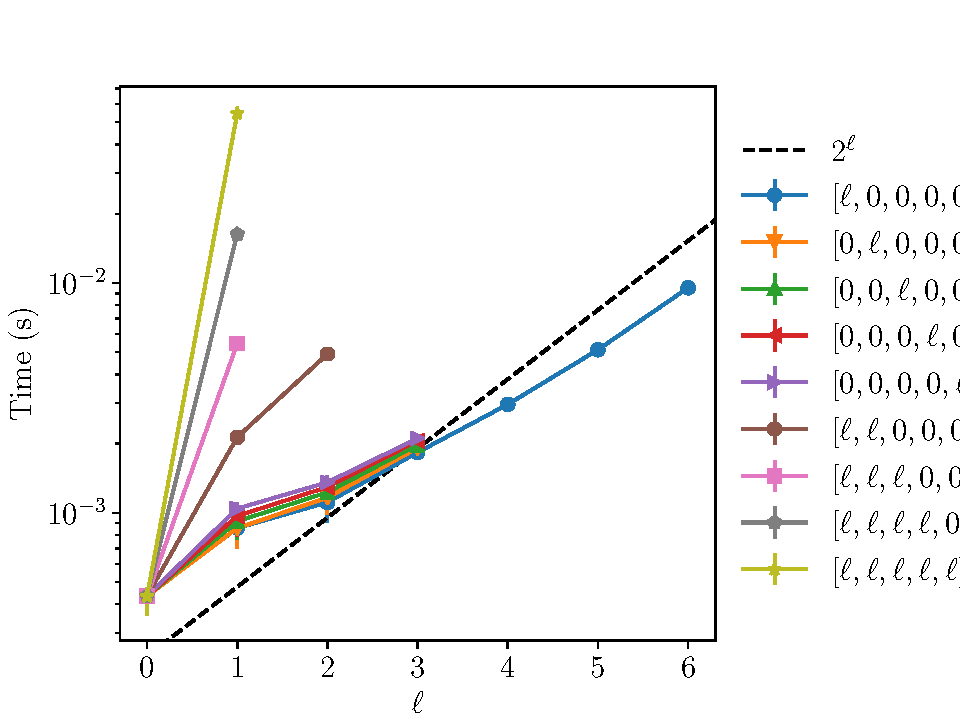
\includegraphics[width=0.95\linewidth]{./figures/rbergomi_8_steps_K_e__4/level_work.pdf}
		\caption{Average Computational time per level}
		\label{fig:misc_rbergomi_8_steps_sub3}
	\end{subfigure}%
	\begin{subfigure}{.5\textwidth}
		\centering
		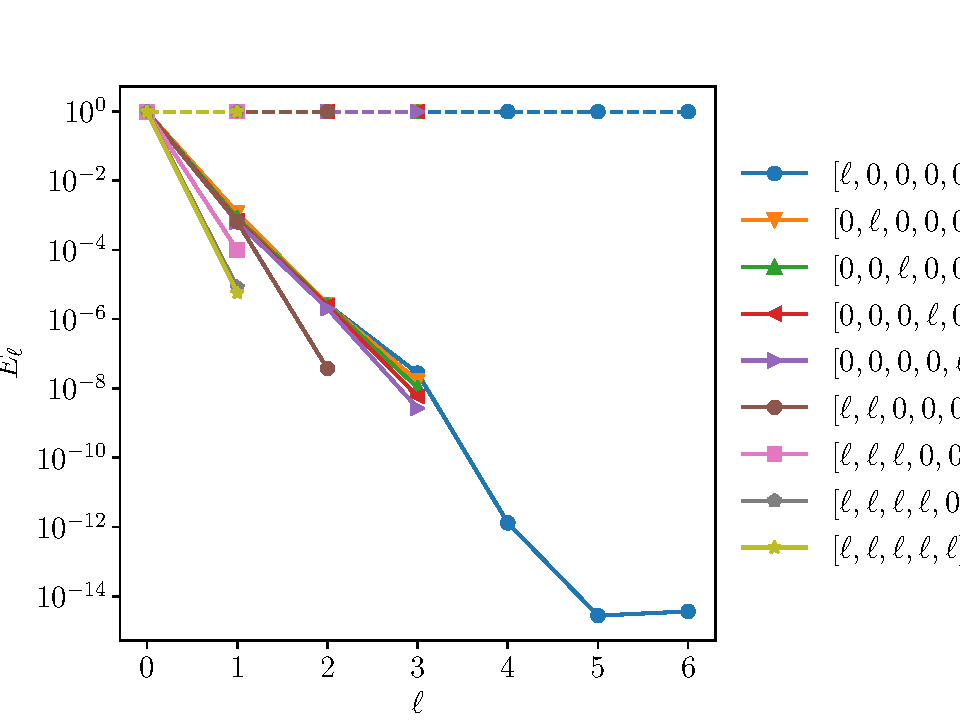
\includegraphics[width=0.95\linewidth]{./figures/rbergomi_8_steps_K_e__4/levels_error_rate.pdf}
		\caption{  The convergence rate of mixed differences per level}
		\label{fig:misc_rbergomi_8_steps_sub4}
	\end{subfigure}%
	\caption{Convergence and work rates for discretization levels  the call payoff with rBergomi model.}
	\label{fig:misc_rbergomi_8_steps_2}
\end{figure}



\newpage
\subsubsection*{Case of $8$ time steps, $K=1.2$}
\begin{figure}[!h]
	\centering
	\begin{subfigure}{.5\textwidth}
		\centering
		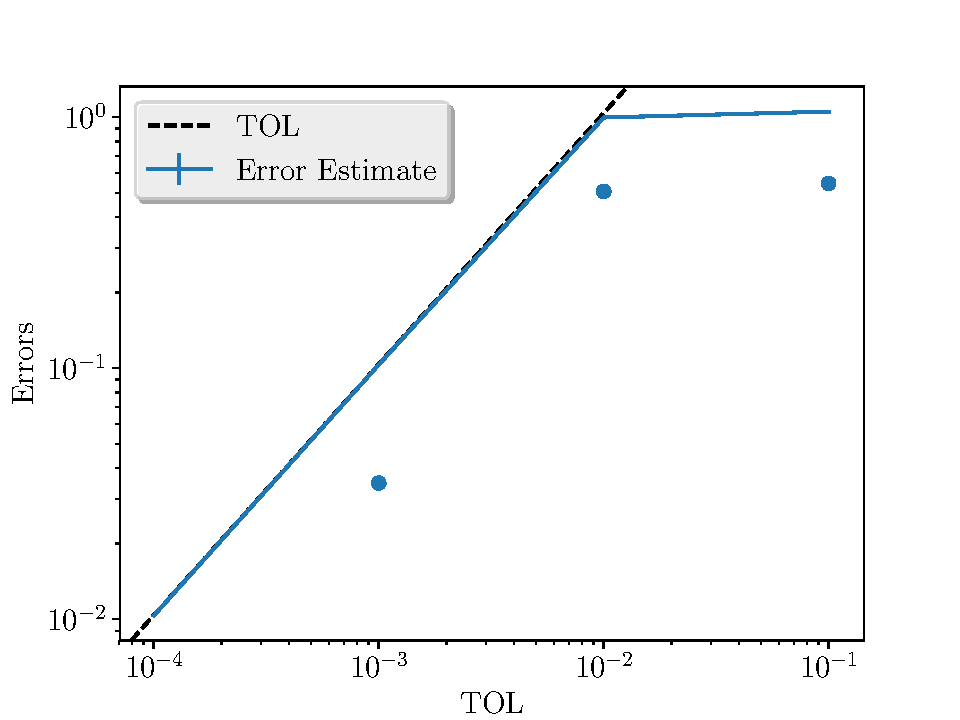
\includegraphics[width=1\linewidth]{./figures/rbergomi_8_steps_K_1_2/error_estimate.pdf}
		\caption{Error estimate}
		\label{fig:misc_rbergomi_8_steps_K_1_2_sub1}
	\end{subfigure}%
	\begin{subfigure}{.5\textwidth}
		\centering
		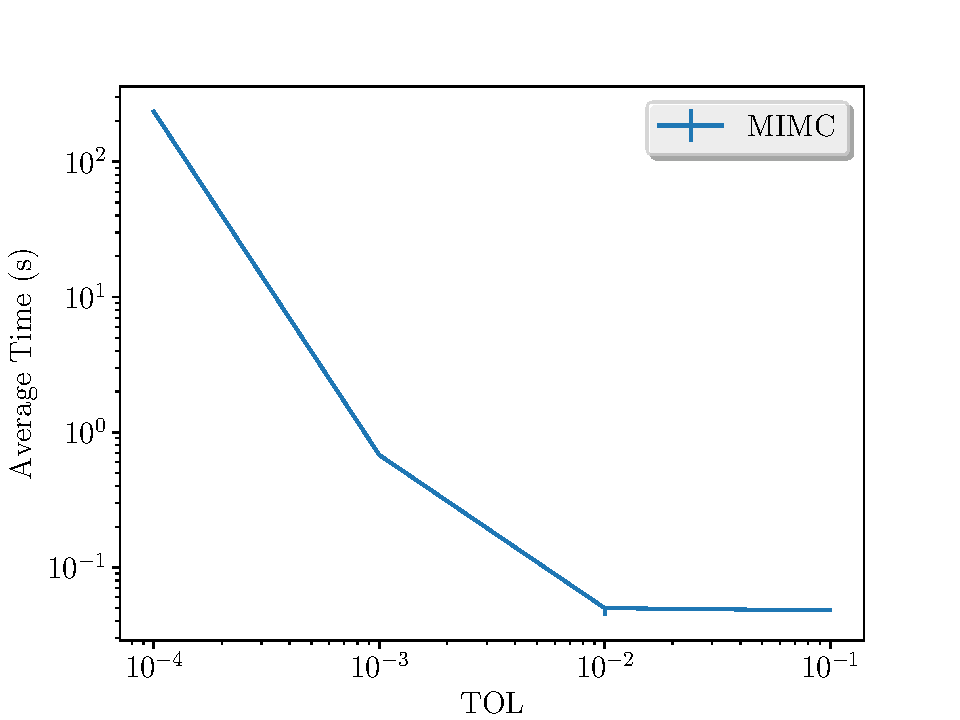
\includegraphics[width=1\linewidth]{./figures/rbergomi_8_steps_K_1_2/average_running_time.pdf}
		\caption{Average running time as a function of $TOL$}
		\label{fig:misc_rbergomi_8_steps_K_1_2_sub2}
	\end{subfigure}%
	\caption{Convergence and complexity results for the call payoff with rBergomi model.}
	\label{fig:misc_rbergomi_8_steps_K_1_2_1}
\end{figure}



\begin{figure}[!h]
	\centering
	\begin{subfigure}{.5\textwidth}
		\centering
		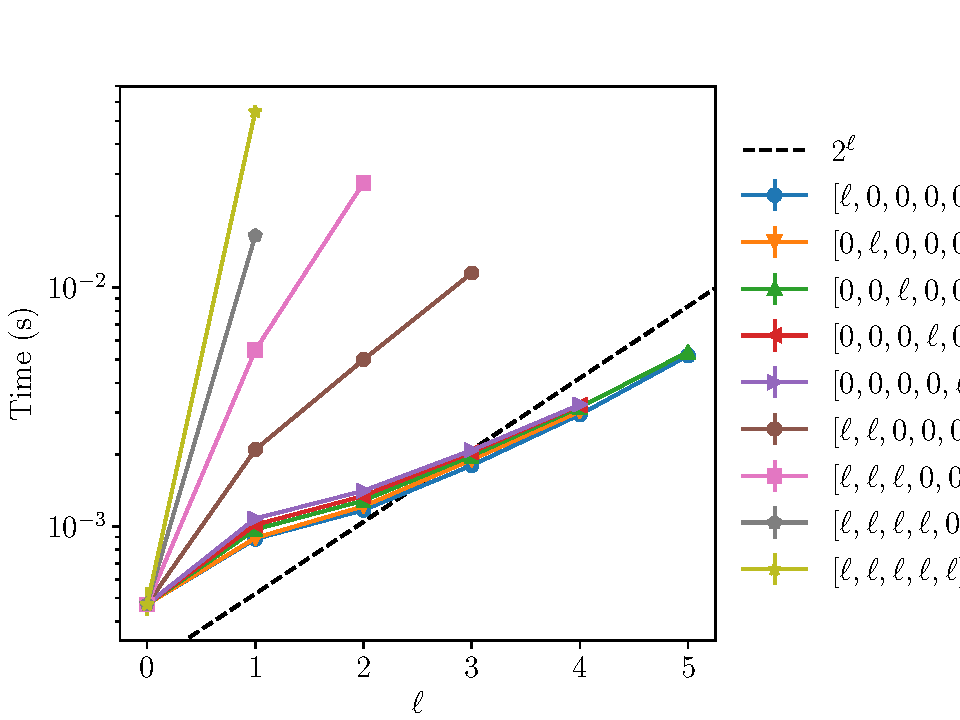
\includegraphics[width=0.95\linewidth]{./figures/rbergomi_8_steps_K_1_2/level_work.pdf}
		\caption{Average Computational time per level}
		\label{fig:misc_rbergomi_8_steps_K_1_2_sub3}
	\end{subfigure}%
	\begin{subfigure}{.5\textwidth}
		\centering
		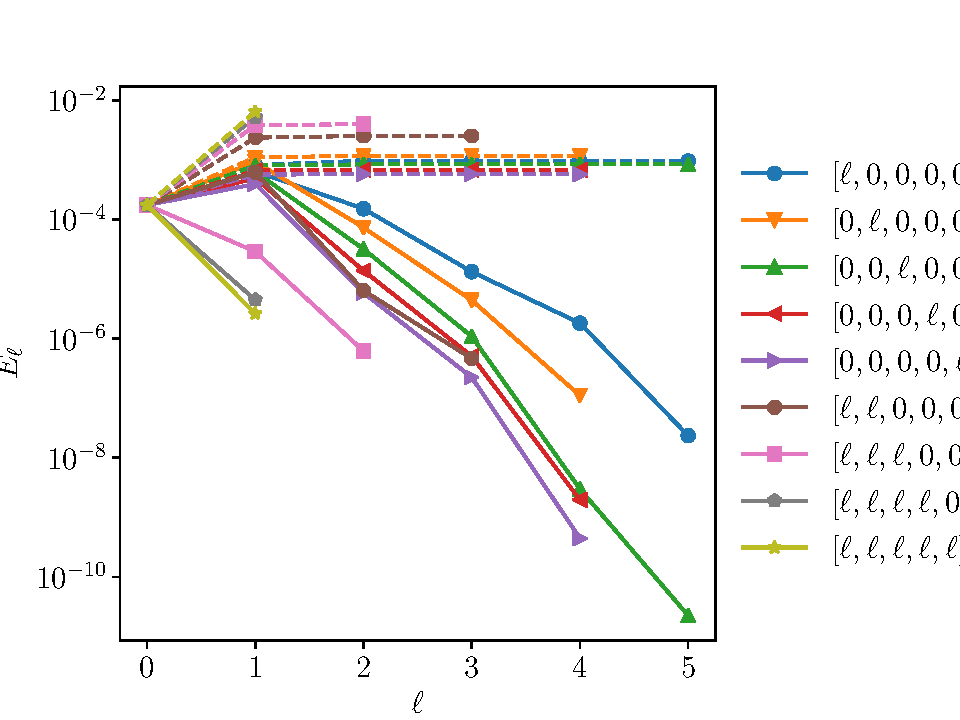
\includegraphics[width=0.95\linewidth]{./figures/rbergomi_8_steps_K_1_2/levels_error_rate.pdf}
		\caption{  The convergence rate of mixed differences per level}
		\label{fig:misc_rbergomi_8_steps_K_1_2_sub4}
	\end{subfigure}%
	\caption{Convergence and work rates for discretization levels  the call payoff with rBergomi model.}
	\label{fig:misc_rbergomi_8_steps_K_1_2_2}
\end{figure}


\newpage
\subsubsection*{Case of $16$ time steps, $K=e^{-4}$}
\begin{figure}[!h]
	\centering
	\begin{subfigure}{.5\textwidth}
		\centering
		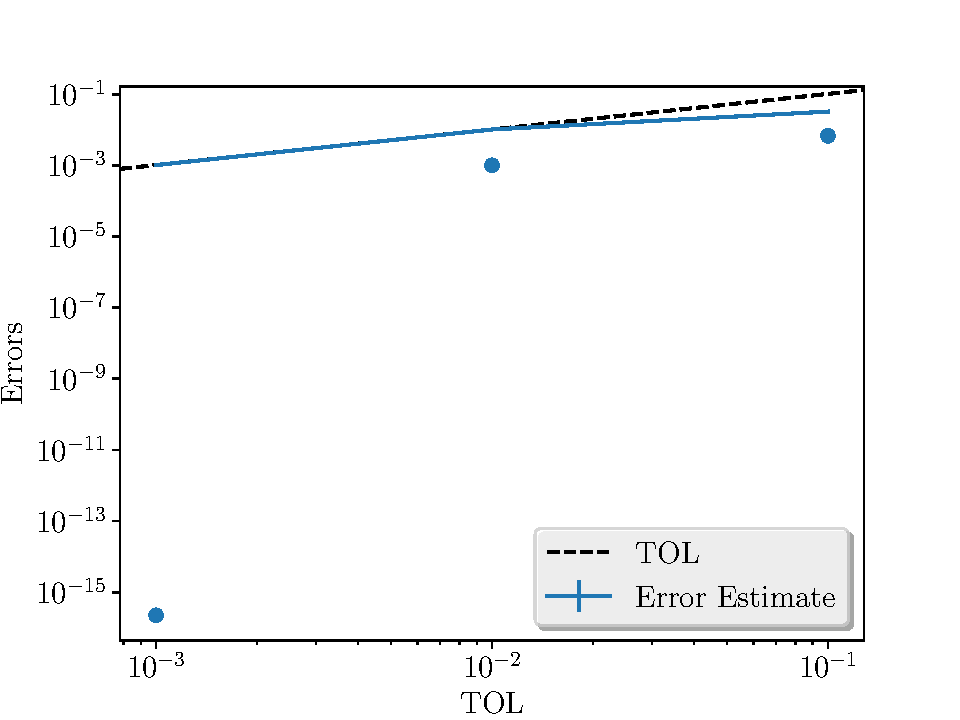
\includegraphics[width=1\linewidth]{./figures/rbergomi_16_steps_K_e__4/error_estimate.pdf}
		\caption{Error estimate}
		\label{fig:misc_rbergomi_16_steps_sub1}
	\end{subfigure}%
	\begin{subfigure}{.5\textwidth}
		\centering
		\includegraphics[width=1\linewidth]{./figures/rbergomi_16_steps_K_e__4/average_running_time.pdf}
		\caption{Average running time as a function of $TOL$}
		\label{fig:misc_rbergomi_16_steps_sub2}
	\end{subfigure}%
	\caption{Convergence and complexity results for the call payoff with rBergomi model.}
	\label{fig:misc_rbergomi_16_steps_1}
\end{figure}



\begin{figure}[!h]
	\centering
	\begin{subfigure}{.5\textwidth}
		\centering
		\includegraphics[width=0.95\linewidth]{./figures/rbergomi_16_steps_K_e__4/level_work.pdf}
		\caption{Average Computational time per level}
		\label{fig:misc_rbergomi_16_steps_sub3}
	\end{subfigure}%
	\begin{subfigure}{.5\textwidth}
		\centering
		\includegraphics[width=0.95\linewidth]{./figures/rbergomi_16_steps_K_e__4/levels_error_rate.pdf}
		\caption{  The convergence rate of mixed differences per level}
		\label{fig:misc_rbergomi_16_steps_sub4}
	\end{subfigure}%
	\caption{Convergence and work rates for discretization levels  the call payoff with rBergomi model.}
	\label{fig:misc_rbergomi_16_steps_2}
\end{figure}


\newpage

\subsubsection*{Case of $16$ time steps, $K=1.2$}
\begin{figure}[!h]
	\centering
	\begin{subfigure}{.5\textwidth}
		\centering
		\includegraphics[width=1\linewidth]{./figures/rbergomi_16_steps_K_1_2/error_estimate.pdf}
		\caption{Error estimate}
		\label{fig:misc_rbergomi_16_steps_K_1_2_sub1}
	\end{subfigure}%
	\begin{subfigure}{.5\textwidth}
		\centering
		\includegraphics[width=1\linewidth]{./figures/rbergomi_16_steps_K_1_2/average_running_time.pdf}
		\caption{Average running time as a function of $TOL$}
		\label{fig:misc_rbergomi_16_steps_K_1_2_sub2}
	\end{subfigure}%
	\caption{Convergence and complexity results for the call payoff with rBergomi model.}
	\label{fig:misc_rbergomi_16_steps_K_1_2_1}
\end{figure}



\begin{figure}[!h]
	\centering
	\begin{subfigure}{.5\textwidth}
		\centering
		\includegraphics[width=0.95\linewidth]{./figures/rbergomi_16_steps_K_1_2/level_work.pdf}
		\caption{Average Computational time per level}
		\label{fig:misc_rbergomi_16_steps_K_1_2_sub3}
	\end{subfigure}%
	\begin{subfigure}{.5\textwidth}
		\centering
		\includegraphics[width=0.95\linewidth]{./figures/rbergomi_16_steps_K_1_2/levels_error_rate.pdf}
		\caption{  The convergence rate of mixed differences per level}
		\label{fig:misc_rbergomi_16_steps_K_1_2_sub4}
	\end{subfigure}%
	\caption{Convergence and work rates for discretization levels  the call payoff with rBergomi model.}
	\label{fig:misc_rbergomi_16_steps_K_1_2_2}
\end{figure}

 %%%%%%%%%%%%%%%%%%%%%%%%%%%%%%%%%%%%%%%%%%
%References
%%%%%%%%%%%%%%%%%%%%%%%%%%%%%%%%%%%%%%%%%%
\newpage
\bibliographystyle{plain}
\bibliography{smoothing} 
\end{document}
